\documentclass[
  man,
  floatsintext,
  longtable,
  nolmodern,
  notxfonts,
  notimes,
  colorlinks=true,linkcolor=blue,citecolor=blue,urlcolor=blue]{apa7}

\usepackage{amsmath}
\usepackage{amssymb}



\usepackage[bidi=default]{babel}
\babelprovide[main,import]{english}


% get rid of language-specific shorthands (see #6817):
\let\LanguageShortHands\languageshorthands
\def\languageshorthands#1{}

\RequirePackage{longtable}
\RequirePackage{threeparttablex}

\makeatletter
\renewcommand{\paragraph}{\@startsection{paragraph}{4}{\parindent}%
	{0\baselineskip \@plus 0.2ex \@minus 0.2ex}%
	{-.5em}%
	{\normalfont\normalsize\bfseries\typesectitle}}

\renewcommand{\subparagraph}[1]{\@startsection{subparagraph}{5}{0.5em}%
	{0\baselineskip \@plus 0.2ex \@minus 0.2ex}%
	{-\z@\relax}%
	{\normalfont\normalsize\bfseries\itshape\hspace{\parindent}{#1}\textit{\addperi}}{\relax}}
\makeatother




\usepackage{longtable, booktabs, multirow, multicol, colortbl, hhline, caption, array, float, xpatch}
\setcounter{topnumber}{2}
\setcounter{bottomnumber}{2}
\setcounter{totalnumber}{4}
\renewcommand{\topfraction}{0.85}
\renewcommand{\bottomfraction}{0.85}
\renewcommand{\textfraction}{0.15}
\renewcommand{\floatpagefraction}{0.7}

\usepackage{tcolorbox}
\tcbuselibrary{listings,theorems, breakable, skins}
\usepackage{fontawesome5}

\definecolor{quarto-callout-color}{HTML}{909090}
\definecolor{quarto-callout-note-color}{HTML}{0758E5}
\definecolor{quarto-callout-important-color}{HTML}{CC1914}
\definecolor{quarto-callout-warning-color}{HTML}{EB9113}
\definecolor{quarto-callout-tip-color}{HTML}{00A047}
\definecolor{quarto-callout-caution-color}{HTML}{FC5300}
\definecolor{quarto-callout-color-frame}{HTML}{ACACAC}
\definecolor{quarto-callout-note-color-frame}{HTML}{4582EC}
\definecolor{quarto-callout-important-color-frame}{HTML}{D9534F}
\definecolor{quarto-callout-warning-color-frame}{HTML}{F0AD4E}
\definecolor{quarto-callout-tip-color-frame}{HTML}{02B875}
\definecolor{quarto-callout-caution-color-frame}{HTML}{FD7E14}

%\newlength\Oldarrayrulewidth
%\newlength\Oldtabcolsep


\usepackage{hyperref}




\providecommand{\tightlist}{%
  \setlength{\itemsep}{0pt}\setlength{\parskip}{0pt}}
\usepackage{longtable,booktabs,array}
\usepackage{calc} % for calculating minipage widths
% Correct order of tables after \paragraph or \subparagraph
\usepackage{etoolbox}
\makeatletter
\patchcmd\longtable{\par}{\if@noskipsec\mbox{}\fi\par}{}{}
\makeatother
% Allow footnotes in longtable head/foot
\IfFileExists{footnotehyper.sty}{\usepackage{footnotehyper}}{\usepackage{footnote}}
\makesavenoteenv{longtable}

\usepackage{graphicx}
\makeatletter
\newsavebox\pandoc@box
\newcommand*\pandocbounded[1]{% scales image to fit in text height/width
  \sbox\pandoc@box{#1}%
  \Gscale@div\@tempa{\textheight}{\dimexpr\ht\pandoc@box+\dp\pandoc@box\relax}%
  \Gscale@div\@tempb{\linewidth}{\wd\pandoc@box}%
  \ifdim\@tempb\p@<\@tempa\p@\let\@tempa\@tempb\fi% select the smaller of both
  \ifdim\@tempa\p@<\p@\scalebox{\@tempa}{\usebox\pandoc@box}%
  \else\usebox{\pandoc@box}%
  \fi%
}
% Set default figure placement to htbp
\def\fps@figure{htbp}
\makeatother


% definitions for citeproc citations
\NewDocumentCommand\citeproctext{}{}
\NewDocumentCommand\citeproc{mm}{%
  \begingroup\def\citeproctext{#2}\cite{#1}\endgroup}
\makeatletter
 % allow citations to break across lines
 \let\@cite@ofmt\@firstofone
 % avoid brackets around text for \cite:
 \def\@biblabel#1{}
 \def\@cite#1#2{{#1\if@tempswa , #2\fi}}
\makeatother
\newlength{\cslhangindent}
\setlength{\cslhangindent}{1.5em}
\newlength{\csllabelwidth}
\setlength{\csllabelwidth}{3em}
\newenvironment{CSLReferences}[2] % #1 hanging-indent, #2 entry-spacing
 {\begin{list}{}{%
  \setlength{\itemindent}{0pt}
  \setlength{\leftmargin}{0pt}
  \setlength{\parsep}{0pt}
  % turn on hanging indent if param 1 is 1
  \ifodd #1
   \setlength{\leftmargin}{\cslhangindent}
   \setlength{\itemindent}{-1\cslhangindent}
  \fi
  % set entry spacing
  \setlength{\itemsep}{#2\baselineskip}}}
 {\end{list}}
\usepackage{calc}
\newcommand{\CSLBlock}[1]{\hfill\break\parbox[t]{\linewidth}{\strut\ignorespaces#1\strut}}
\newcommand{\CSLLeftMargin}[1]{\parbox[t]{\csllabelwidth}{\strut#1\strut}}
\newcommand{\CSLRightInline}[1]{\parbox[t]{\linewidth - \csllabelwidth}{\strut#1\strut}}
\newcommand{\CSLIndent}[1]{\hspace{\cslhangindent}#1}





\usepackage{newtx}

\defaultfontfeatures{Scale=MatchLowercase}
\defaultfontfeatures[\rmfamily]{Ligatures=TeX,Scale=1}





\title{Education Funding Inequality and Academic Performance Disparity
between Migrant and Local Students in China}


\shorttitle{D2MR Final Project}


\usepackage{etoolbox}






\author{Jiayi Zou}



\affiliation{
{MA Program in the Social Sciences, University of Chicago}}




\leftheader{Zou}



\abstract{Internal migration is an unique social problem for urban
governance in China One of the major issue is the underperformance of
migrant children in schools, and fiscal decentralization and the Hukou
system restricts them from benefiting from the equal level of education
finance as their local counterparts do. How governments' differentiated
provision of education fundings affects the academic performance
disparity between migrant students and local students in China? Applying
multilevel model, we found that after clustering two groups of students
by school ids, migrant status can benefit migrant students' performance
in Chinese exam, while their academic performance across three subjects
can decrease due to excluding enrollment of migrants, lower quota of
per-student funding, and missing information in subsidies and fiscal
allocation. }

\keywords{education inequality, internal migration, education
funding, fiscal decentralization}

\authornote{ 

\par{  This project is the final assignment for Data to Manuscript in R
(D2MR) instructed by Dr.~Natalie Dowling. It also serves as an interim
result of Jiayi Zou's MA thesis project.   The author is grateful
Dr.~Dowling for supporting this project and offering guidance throughout
the quarter.  }
\par{Correspondence concerning this article should be addressed to Jiayi
Zou, MA Program in the Social Sciences, University of Chicago, 1155 E
60th St., Chicago, IL 60637, USA, Email: jiayizou@uchicago.edu}
}

\makeatletter
\let\endoldlt\endlongtable
\def\endlongtable{
\hline
\endoldlt
}
\makeatother

\urlstyle{same}



\usepackage{fontspec}
\usepackage{multirow}
\usepackage{multicol}
\usepackage{colortbl}
\usepackage{hhline}
\newlength\Oldarrayrulewidth
\newlength\Oldtabcolsep
\usepackage{longtable}
\usepackage{array}
\usepackage{hyperref}
\usepackage{float}
\usepackage{wrapfig}
\usepackage{booktabs}
\usepackage{pdflscape}
\usepackage{tabu}
\usepackage{threeparttable}
\usepackage{threeparttablex}
\usepackage[normalem]{ulem}
\usepackage{makecell}
\usepackage{xcolor}
\makeatletter
\@ifpackageloaded{caption}{}{\usepackage{caption}}
\AtBeginDocument{%
\ifdefined\contentsname
  \renewcommand*\contentsname{Table of contents}
\else
  \newcommand\contentsname{Table of contents}
\fi
\ifdefined\listfigurename
  \renewcommand*\listfigurename{List of Figures}
\else
  \newcommand\listfigurename{List of Figures}
\fi
\ifdefined\listtablename
  \renewcommand*\listtablename{List of Tables}
\else
  \newcommand\listtablename{List of Tables}
\fi
\ifdefined\figurename
  \renewcommand*\figurename{Figure}
\else
  \newcommand\figurename{Figure}
\fi
\ifdefined\tablename
  \renewcommand*\tablename{Table}
\else
  \newcommand\tablename{Table}
\fi
}
\@ifpackageloaded{float}{}{\usepackage{float}}
\floatstyle{ruled}
\@ifundefined{c@chapter}{\newfloat{codelisting}{h}{lop}}{\newfloat{codelisting}{h}{lop}[chapter]}
\floatname{codelisting}{Listing}
\newcommand*\listoflistings{\listof{codelisting}{List of Listings}}
\makeatother
\makeatletter
\makeatother
\makeatletter
\@ifpackageloaded{caption}{}{\usepackage{caption}}
\@ifpackageloaded{subcaption}{}{\usepackage{subcaption}}
\makeatother

% From https://tex.stackexchange.com/a/645996/211326
%%% apa7 doesn't want to add appendix section titles in the toc
%%% let's make it do it
\makeatletter
\xpatchcmd{\appendix}
  {\par}
  {\addcontentsline{toc}{section}{\@currentlabelname}\par}
  {}{}
\makeatother

%% Disable longtable counter
%% https://tex.stackexchange.com/a/248395/211326

\usepackage{etoolbox}

\makeatletter
\patchcmd{\LT@caption}
  {\bgroup}
  {\bgroup\global\LTpatch@captiontrue}
  {}{}
\patchcmd{\longtable}
  {\par}
  {\par\global\LTpatch@captionfalse}
  {}{}
\apptocmd{\endlongtable}
  {\ifLTpatch@caption\else\addtocounter{table}{-1}\fi}
  {}{}
\newif\ifLTpatch@caption
\makeatother

\begin{document}

\maketitle


\setcounter{secnumdepth}{-\maxdimen} % remove section numbering

\setlength\LTleft{0pt}


\section{Introduction}\label{introduction}

Internal migration in China has accelerated along with urbanization
since the implementation of Reform and Opening Up policy in the early
1980s. Statistics from the 7th National Census in 2020 show that over 70
million children in China have migration status, which means one fourth
of Chinese child population move interprovincially or intraprovincially
with their parents \footnote{See in
  \href{https://www.163.com/dy/article/JHFCU34705560ZWH.html}{Promoting
  reunion and avoiding separation - China's migrant children development
  report 2024}.}. Education and sociology research focusing on internal
migrant students found that these children have a relatively lower
school achievement compared to local students without migrant status,
and suffer from academic and financial difficulties, as well as
alienation in public education system
(\citeproc{ref-chenAccessPublicSchools2013}{Chen \& Feng, 2013};
\citeproc{ref-huangMythMigrantsProblems2017a}{Huang, 2017}).

Previous studies offered policy explanations for migrant students'
underachievement. Li (\citeproc{ref-liDataAnalysisCurrent2018}{2018})
indicated that central governments have less educational funding
distributed to provinces containing more migrant population due to
fiscal decentralization. On the other hand, the \emph{Hukou} policy
\footnote{The \emph{Hukou} Policy is a population management policy that
  restraints non-local residents from/uplifts the threshold of enjoying
  the same social, medical, and educational public services as local
  households do.} has a history of limiting policy supports for internal
migrants including subsidies, fee standards, and other financial
accesses, which contributes migrant students' underperformance in school
(\citeproc{ref-luVillagersCityResilience2023}{Lu, 2023}).

However, both perspectives have failed to identify an integrated
framework: if we can discover the impact of differentiated financial
supports and per student funding appropriated to two groups of students,
then it is plausible to assume that fiscal decentralization is producing
local-migrant educational inequity through the lens of \emph{Hukou}
status.

In this study, I seek to understand \textbf{how governments'
differentiated provision of education fundings affects the academic
performance disparity between migrant students and local students in
China} . My hypothesis is \textbf{when the government provides migrant
students with limited fundings, and less-supportive charging standards
and subsidy policies, the academic performance gap between the two
groups of students is likely to widen}.

Beyond measuring educational disparities created by the complexity of
fiscal decentralization and population management system, this research
has practical significance for addressing the ongoing migrant problems
in China's urban governance and the institution of compulsory education
(\citeproc{ref-nationalbureauofstatisticsofchinaetal_2023_what}{National
Bureau of Statistics of China et al., 2023}). Last but not least, this
study can also offer indications for how educational finance and
policies provided by government interacts with structural inequality in
other social contexts (e.g., areas with higher poverty level or racial
disparities, see in studies by Baird
(\citeproc{ref-baird_2008_federal}{2008}) and Hyman
(\citeproc{ref-hyman_2017_does}{2017})).

\section{Literature Review}\label{literature-review}

In this study, we define \emph{provision of education fundings} as a
combination of three elements: (1) the amount of funding, including
per-student funding, subsidies, and charging standards; (2) the
proportion of funding, which is seperated into central/provincial and
county/district level; and (3) the indicator of differentiation, which
is whether migrant students enjoy the equal educational financial
resources as locally-registered students in terms of funding, subsidies,
and charging standards. Inspired by Knoeppel and Della Sala
(\citeproc{ref-knoeppelEducationFundingStudent2015}{2015}), we consider
that education funding, influenced by fiscal decentralization and
\emph{Hukou} system, affects migrant and local students in the same
schools through context for schooling, which results in unequal academic
performances between two student groups.

\subsection{Education Funding and Academic
Achievement}\label{education-funding-and-academic-achievement}

Scholarship in education funding suggests that students of color have
been continuously underfunded by federal and state, and the discrepancy
between their and higher-SES/white counterparts' academic performance
persists (\citeproc{ref-darling-hammond_2004_color}{Darling-Hammond,
2004}; \citeproc{ref-gaddislauen_2014_school}{Gaddis \& Lauen, 2014};
\citeproc{ref-lafortuneetal_2018_school}{Lafortune et al., 2018};
\citeproc{ref-ryan_1999_schools}{Ryan, 1999}). In China, researchers
found similar patterns and disparities among migrant students and
local-\emph{Hukou} students. Evidence from China Education Paney survey
indicates that local students outperform migrant students at higher
quantile point, and increasing total education expenditure is likely
shrink the academic achievement gap
(\citeproc{ref-fangStudyOutcomeEquity2024}{Fang \& Zhang, 2024}).
However, the association between other aspects of education expenditure
(e.g.~per student funding, central and local government appropriation
ratio) and local-migrant academic outcome equity requires further
exploration, as most studies center on how funding expands spatial
education inequity rather than disparities between different
\emph{Hukou} statuses in cities
(\citeproc{ref-weiAnalysisReportUrbanrural2022}{Wei et al., 2022}).

\subsection{Fiscal Decentralization and Descriminatory Policies against
Internal
Migrants}\label{fiscal-decentralization-and-descriminatory-policies-against-internal-migrants}

Beyond education finance disparities, education policies also differ for
migrant and local students in many provinces, which means students
without local registration (\emph{hukou}) may have no government
subsidies or face different charging standards. Researchers refer this
phenomenon as deflecting internal migrants' demands and using education
to control urban population influx
(\citeproc{ref-chanPhantomServicesDeflecting2019}{Chan \& O'Brien,
2019}; \citeproc{ref-friedmanBiopoliticsUrbanizationChina2018}{Friedman,
2018}). The disadvantage encountered by migran students varies in
different city scenarios: if local education policy background is more
\emph{Hukou}-based discriminatory, then migrant students are more likely
to receive lower school performance than local students
(\citeproc{ref-maMigrantStatusSchool2020}{Ma, 2020}). Deflecting
education resources away from the underprivileged students occurs in
U.S. schools to avoid losing fundings under school accountability, as
the minority subgroups have a higher possibility to fall short of the
average academic target
(\citeproc{ref-hanushekraymond_2005_does}{Hanushek \& Raymond, 2005};
\citeproc{ref-oday_2009_complexity}{O'Day, 2009}). Similarly, turning
down education fundings for migrant students is also a strategy for
Chinese local governments to decrease overall financial stress due to
fiscal decentralization
(\citeproc{ref-jinRegionalDecentralizationFiscal2005a}{Jin et al.,
2005}; \citeproc{ref-longFiscalDecentralisationKnowledge2017}{Long et
al., 2017}).

As migrant students represent social minorities with limited or without
\emph{Hukou}-related rights in urban spaces, exploring their education
achievements influenced by government funding and financial supports can
demonstrate the dynamic and diverse efficiency of providing public
services, offering empirical evidence for the development of
decentralization theory
(\citeproc{ref-oatesSecondGenerationTheoryFiscal2005}{Oates, 2005},
\citeproc{ref-oates_2008_evolution}{2008}).

\section{Data and Methods}\label{data-and-methods}

\subsection{Data}\label{data}

In this project, we use the follow-up (2014-2015) dataset from the China
Education Panel Survey
\href{http://ceps.ruc.edu.cn/English/Home.htm}{CEPS}. CEPS is conducted
by National Survey Research Center at Renmin University of China and it
is the most used dataset in studies of Chinese internal migrant
students. Data includes 1769 migrant students and 7960 non-migrant
students who have were at 9th Grade as in the final year of Junior High.
We will merge datasets based on student, class, and school id, and
remove values without valid information of hukou status.

\subsection{Measures}\label{measures}

The dependent variable in our study is the academic performance, which
is measured by three indexes: score (percentage) of Chinese,
Mathematics, and English exams. Table~\ref{tbl-summary-w2clean} shows
the mean, standardized deviation and number of per-student funding
categorized by student groups.

\begin{table}

{\caption{{Summary Results of per-student
funding}{\label{tbl-summary-w2clean}}}
\vspace{-20pt}}

\global\setlength{\Oldarrayrulewidth}{\arrayrulewidth}

\global\setlength{\Oldtabcolsep}{\tabcolsep}

\setlength{\tabcolsep}{2pt}

\renewcommand*{\arraystretch}{1.5}



\providecommand{\ascline}[3]{\noalign{\global\arrayrulewidth #1}\arrayrulecolor[HTML]{#2}\cline{#3}}

\begin{longtable*}[c]{|p{0.75in}|p{0.75in}|p{0.75in}|p{0.75in}}



\ascline{0.75pt}{000000}{1-4}

\multicolumn{1}{>{\centering}m{\dimexpr 0.75in+0\tabcolsep}}{\textcolor[HTML]{000000}{\fontsize{11}{22}\selectfont{\global\setmainfont{Times New Roman}{Migrant\ status}}}} & \multicolumn{1}{>{\centering}m{\dimexpr 0.75in+0\tabcolsep}}{\textcolor[HTML]{000000}{\fontsize{11}{22}\selectfont{\global\setmainfont{Times New Roman}{MPG\ (mean)}}}} & \multicolumn{1}{>{\centering}m{\dimexpr 0.75in+0\tabcolsep}}{\textcolor[HTML]{000000}{\fontsize{11}{22}\selectfont{\global\setmainfont{Times New Roman}{MPG\ (sd)}}}} & \multicolumn{1}{>{\centering}m{\dimexpr 0.75in+0\tabcolsep}}{\textcolor[HTML]{000000}{\fontsize{11}{22}\selectfont{\global\setmainfont{Times New Roman}{N}}}} \\

\ascline{0.75pt}{000000}{1-4}\endfirsthead 

\ascline{0.75pt}{000000}{1-4}

\multicolumn{1}{>{\centering}m{\dimexpr 0.75in+0\tabcolsep}}{\textcolor[HTML]{000000}{\fontsize{11}{22}\selectfont{\global\setmainfont{Times New Roman}{Migrant\ status}}}} & \multicolumn{1}{>{\centering}m{\dimexpr 0.75in+0\tabcolsep}}{\textcolor[HTML]{000000}{\fontsize{11}{22}\selectfont{\global\setmainfont{Times New Roman}{MPG\ (mean)}}}} & \multicolumn{1}{>{\centering}m{\dimexpr 0.75in+0\tabcolsep}}{\textcolor[HTML]{000000}{\fontsize{11}{22}\selectfont{\global\setmainfont{Times New Roman}{MPG\ (sd)}}}} & \multicolumn{1}{>{\centering}m{\dimexpr 0.75in+0\tabcolsep}}{\textcolor[HTML]{000000}{\fontsize{11}{22}\selectfont{\global\setmainfont{Times New Roman}{N}}}} \\

\ascline{0.75pt}{000000}{1-4}\endhead



\multicolumn{1}{>{\centering}m{\dimexpr 0.75in+0\tabcolsep}}{\textcolor[HTML]{000000}{\fontsize{11}{22}\selectfont{\global\setmainfont{Times New Roman}{1}}}} & \multicolumn{1}{>{\centering}m{\dimexpr 0.75in+0\tabcolsep}}{\textcolor[HTML]{000000}{\fontsize{11}{22}\selectfont{\global\setmainfont{Times New Roman}{1,044.41}}}} & \multicolumn{1}{>{\centering}m{\dimexpr 0.75in+0\tabcolsep}}{\textcolor[HTML]{000000}{\fontsize{11}{22}\selectfont{\global\setmainfont{Times New Roman}{675.19}}}} & \multicolumn{1}{>{\centering}m{\dimexpr 0.75in+0\tabcolsep}}{\textcolor[HTML]{000000}{\fontsize{11}{22}\selectfont{\global\setmainfont{Times New Roman}{7,960}}}} \\





\multicolumn{1}{>{\centering}m{\dimexpr 0.75in+0\tabcolsep}}{\textcolor[HTML]{000000}{\fontsize{11}{22}\selectfont{\global\setmainfont{Times New Roman}{2}}}} & \multicolumn{1}{>{\centering}m{\dimexpr 0.75in+0\tabcolsep}}{\textcolor[HTML]{000000}{\fontsize{11}{22}\selectfont{\global\setmainfont{Times New Roman}{1,280.29}}}} & \multicolumn{1}{>{\centering}m{\dimexpr 0.75in+0\tabcolsep}}{\textcolor[HTML]{000000}{\fontsize{11}{22}\selectfont{\global\setmainfont{Times New Roman}{792.98}}}} & \multicolumn{1}{>{\centering}m{\dimexpr 0.75in+0\tabcolsep}}{\textcolor[HTML]{000000}{\fontsize{11}{22}\selectfont{\global\setmainfont{Times New Roman}{1,769}}}} \\

\ascline{0.75pt}{000000}{1-4}



\end{longtable*}



\arrayrulecolor[HTML]{000000}

\global\setlength{\arrayrulewidth}{\Oldarrayrulewidth}

\global\setlength{\tabcolsep}{\Oldtabcolsep}

\renewcommand*{\arraystretch}{1}

{\vspace{-20pt}
\noindent \emph{Note.} Mean, standardized deviation and number of per\_st\_funding}

\end{table}

In Figure~\ref{fig-box-academic-performance}, a primary investigation
into the follow-up dataset suggests that the medium and average of all
three test scores for migrant students are all less than the equivalents
for non-migrant students. Migrant students performances in Chinese and
English exams are more concentrated than local students, but possibly
due to different sample size. More outliers in Chinese exam scores
appeared in migrant student group than their local counterparts,
suggesting migrant students might experience greater difficulty in
achieveing in Chinese exams. Additionally, the average Chinese,
Mathematics and English exam scores of migrant students are respectively
67.6533095, 62.026304, and 60.5801271, which are lower than their local
counterparts' academic achievements (68.6661009, 63.9595634, and
61.9371545).

\begin{figure}

\caption{\label{fig-box-academic-performance}Comparison of the
distribution of Chinese, Mathematics, and English exam scores (Migrant
vs.~Local students)}

\centering{

\pandocbounded{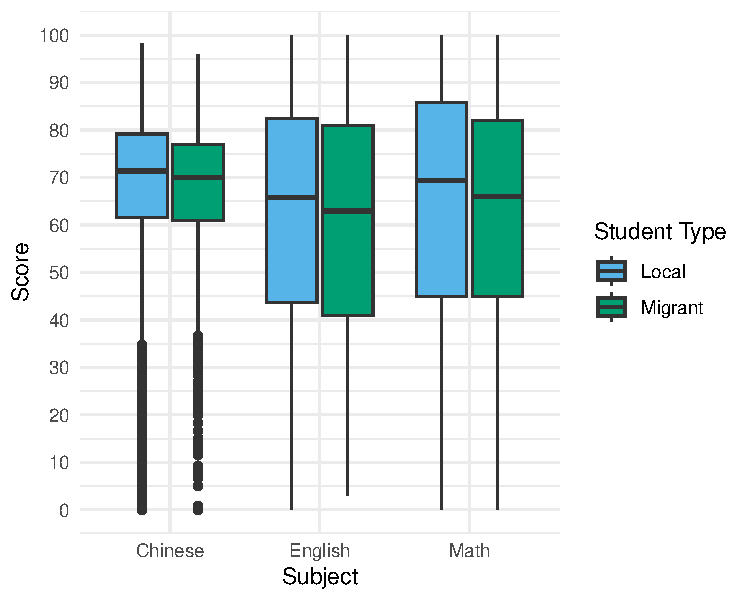
\includegraphics[keepaspectratio]{migrant-student-education_files/figure-pdf/fig-box-academic-performance-1.pdf}}

}

\end{figure}%

As for the independent variable, we take three aspects into account: the
amount of per-student funding; the proportion of funding sources, which
is seperated into central/provincial level and county/district level;
and whether migrant students enjoy the equal funding, subsidies, and
charging standards as locally-registered students do.

\begin{table}

{\caption{{}{\label{tbl-ttest-two-sample-perfunding}}}
\vspace{-20pt}}

\centering
\resizebox{\ifdim\width>\linewidth\linewidth\else\width\fi}{!}{
\begin{tabular}{lrrrrr}
\toprule
  & Statistic (t) & df & P-value & Mean (Local students) & Mean (Migrant students)\\
\midrule
t & -11.6108 & 2369.945 & 0 & 1044.407 & 1280.291\\
\bottomrule
\end{tabular}}

\end{table}

In Table~\ref{tbl-ttest-two-sample-perfunding}, we examined the
difference of mean per-student funding for local and migrant students.
The results indicate that the average per-student funding is
significantly different in two student subgroups, with a \(p\)-value of
0. It is worth noticing that the mean funding for each migrant student
(1280.29051) is higher than the local student's (1044.4065621), which
aligns with the policy guidance from central government in China. The
result is also counterintuitive with the reverse comparison of academic
achievements in Figure~\ref{fig-box-academic-performance}. These
findings call for further investigation in the the effect of educational
funding provision on academic achievement inequality.

\subsection{Methods}\label{methods}

We employ a \textbf{Multilevel Model (MLM)} to see the effect of
independent variables on the academic performance gap between migrant
students and local students. Since migrant students and local students
are clustered in different schools, MLM can provide a hierarchical model
fitness that can take cluster effect into account
(\citeproc{ref-antonoplisStudyingSocioeconomicStatus2023}{Antonoplis,
2023}). We will implement random intercept, fixed slope model to examine
the research question primarily. When analyzing data in later
procedures, MLM can be adjusted with improvement in significance tests
and improvement in fit. The two-level model can be put in an
incorporated formula:
\[ examscore_{ij}= \beta_0 + \beta_1 \cdot mig\_status + \beta_2 \cdot centgov\_fund\_pct_j + \beta_3 \cdot prefgov\_fund\_pct_j \]
\[+\beta_4 \cdot countgov\_fund\_pct_j + \beta_5 \cdot per\_st\_funding_j + \beta_6 \cdot mig\_funding_j + \beta_7 \cdot same\_charge\_std_j\]
\[ + \beta_8 \cdot mig\_subsidy_j  + \beta_9 \cdot (mig\_status_{ij} \times centgov\_fund\_pct_j) \]
\[ + \beta_{10} \cdot (mig\_status_{ij} \times prefgov\_fund\_pct_j) + \beta_{11} \cdot (mig\_status_{ij} \times countgov\_fund\_pct_j) \]
\[ + \beta_{12} \cdot (mig\_status_{ij} \times per\_st\_funding_j)  + \beta_{13} \cdot (mig\_status_{ij} \times mig\_funding_j) \]
\[ + \beta_{14} \cdot (mig\_status_{ij} \times same\_charge\_std_j)  + \beta_{15} \cdot (mig\_status_{ij} \times mig\_subsidy_j) + u_j + \epsilon_{ij} \]
In this funtion, we denote \emph{i} as the individual student and
\emph{j} as the school. The estimate for the fixed effect are as
follows: (1) \(\beta_0\) is the overall intercept; (2) \(\beta_1\)
stands for the effect of being a migrant student; (3) \(\beta_2\) to
\(\beta_8\) extimate the effects of independent variables; (4)
\(\beta_9\) to \(\beta_15\) extimate the interaction effects of
independent variables and migrant status; (5) \(u_j\) is the random
intercept for school \emph{j}; and (6) \(\epsilon_{ij}\) represents the
residual error.

\section{Analysis Results}\label{analysis-results}

\subsection{Linear Relation between Per-student Funding and Academic
Achievements}\label{linear-relation-between-per-student-funding-and-academic-achievements}

We first investigated the correlation between per-student funding and
exam scores. Figure~\ref{fig-ggplot-funding-score} shows that the linear
relation between per-student funding and academic achievements is
positive across student groups and subjects. The estimate for the
relation of Chinese exam score with per-student funding is relatively
smaller than the other two subjects. However, we cannot observe a
significant difference in this relation between local student and
migrant student groups.

\begin{figure}

\caption{\label{fig-ggplot-funding-score}The linear relation between
per-student funding and exam scores across two student groups}

\centering{

\pandocbounded{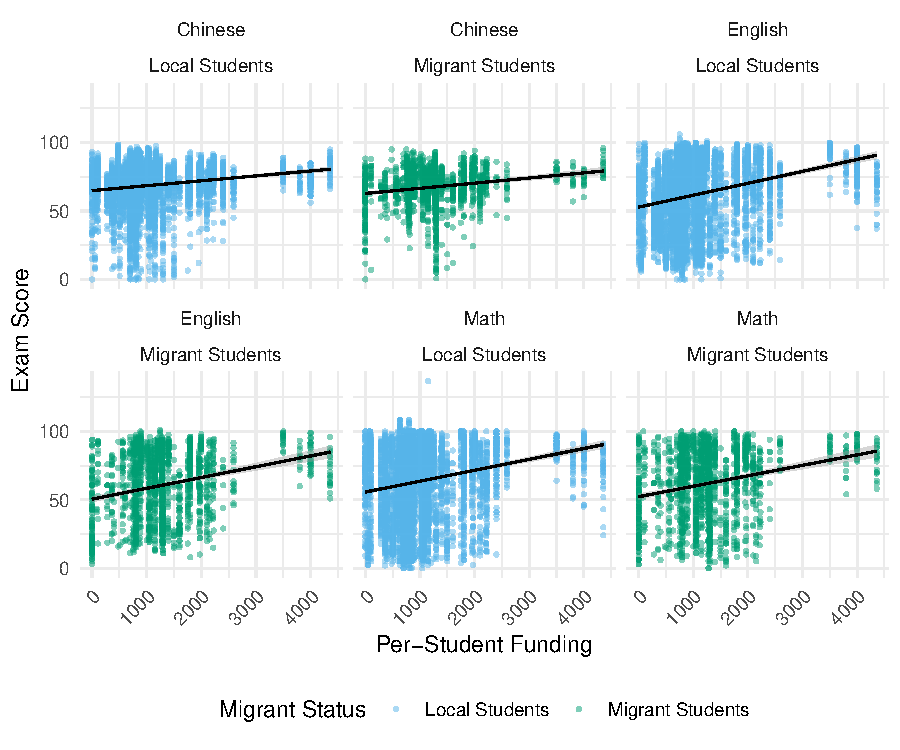
\includegraphics[keepaspectratio]{migrant-student-education_files/figure-pdf/fig-ggplot-funding-score-1.pdf}}

}

\end{figure}%

\subsection{The Effect of Education Funding on Academic Achievments in
Different Student
Groups}\label{the-effect-of-education-funding-on-academic-achievments-in-different-student-groups}

In this section, we employed the MLM method to estimate the effect of
educational funding on the exam scores in three subjects. In the
results, the estimate of the migrant status variable
\texttt{mig\_status} represents \(\beta_1\), which is the effect of
being a migrant student on the overall academic performance. The rest of
the estimates are for the independent variables or interaction terms.

\begin{table}

{\caption{{The effect of education funding on Chinese exam scores
differences within schools}{\label{tbl-chinese-achievement}}}
\vspace{-20pt}}

\global\setlength{\Oldarrayrulewidth}{\arrayrulewidth}

\global\setlength{\Oldtabcolsep}{\tabcolsep}

\setlength{\tabcolsep}{2pt}

\renewcommand*{\arraystretch}{1}



\providecommand{\ascline}[3]{\noalign{\global\arrayrulewidth #1}\arrayrulecolor[HTML]{#2}\cline{#3}}

\begin{longtable*}[c]{cccccc}



\ascline{1.5pt}{666666}{1-6}

\multicolumn{1}{>{}l}{\textcolor[HTML]{000000}{\fontsize{11}{11}\selectfont{\global\setmainfont{Arial}{Term}}}} & \multicolumn{1}{>{}r}{\textcolor[HTML]{000000}{\fontsize{11}{11}\selectfont{\global\setmainfont{Arial}{Estimate}}}} & \multicolumn{1}{>{}r}{\textcolor[HTML]{000000}{\fontsize{11}{11}\selectfont{\global\setmainfont{Arial}{Std.\ Error}}}} & \multicolumn{1}{>{}r}{\textcolor[HTML]{000000}{\fontsize{11}{11}\selectfont{\global\setmainfont{Arial}{df}}}} & \multicolumn{1}{>{}r}{\textcolor[HTML]{000000}{\fontsize{11}{11}\selectfont{\global\setmainfont{Arial}{t.value}}}} & \multicolumn{1}{>{}r}{\textcolor[HTML]{000000}{\fontsize{11}{11}\selectfont{\global\setmainfont{Arial}{P.Value}}}} \\

\ascline{1.5pt}{666666}{1-6}\endfirsthead 

\ascline{1.5pt}{666666}{1-6}

\multicolumn{1}{>{}l}{\textcolor[HTML]{000000}{\fontsize{11}{11}\selectfont{\global\setmainfont{Arial}{Term}}}} & \multicolumn{1}{>{}r}{\textcolor[HTML]{000000}{\fontsize{11}{11}\selectfont{\global\setmainfont{Arial}{Estimate}}}} & \multicolumn{1}{>{}r}{\textcolor[HTML]{000000}{\fontsize{11}{11}\selectfont{\global\setmainfont{Arial}{Std.\ Error}}}} & \multicolumn{1}{>{}r}{\textcolor[HTML]{000000}{\fontsize{11}{11}\selectfont{\global\setmainfont{Arial}{df}}}} & \multicolumn{1}{>{}r}{\textcolor[HTML]{000000}{\fontsize{11}{11}\selectfont{\global\setmainfont{Arial}{t.value}}}} & \multicolumn{1}{>{}r}{\textcolor[HTML]{000000}{\fontsize{11}{11}\selectfont{\global\setmainfont{Arial}{P.Value}}}} \\

\ascline{1.5pt}{666666}{1-6}\endhead



\multicolumn{1}{>{}l}{\textcolor[HTML]{000000}{\fontsize{11}{11}\selectfont{\global\setmainfont{Arial}{(Intercept)}}}} & \multicolumn{1}{>{}r}{\textcolor[HTML]{000000}{\fontsize{11}{11}\selectfont{\global\setmainfont{Arial}{61.576}}}} & \multicolumn{1}{>{}r}{\textcolor[HTML]{000000}{\fontsize{11}{11}\selectfont{\global\setmainfont{Arial}{3.582}}}} & \multicolumn{1}{>{}r}{\textcolor[HTML]{000000}{\fontsize{11}{11}\selectfont{\global\setmainfont{Arial}{119.001}}}} & \multicolumn{1}{>{}r}{\textcolor[HTML]{000000}{\fontsize{11}{11}\selectfont{\global\setmainfont{Arial}{17.193}}}} & \multicolumn{1}{>{}r}{\textcolor[HTML]{000000}{\fontsize{11}{11}\selectfont{\global\setmainfont{Arial}{0.000}}}} \\





\multicolumn{1}{>{}l}{\textcolor[HTML]{000000}{\fontsize{11}{11}\selectfont{\global\setmainfont{Arial}{mig\_status2}}}} & \multicolumn{1}{>{}r}{\textcolor[HTML]{000000}{\fontsize{11}{11}\selectfont{\global\setmainfont{Arial}{3.806}}}} & \multicolumn{1}{>{}r}{\textcolor[HTML]{000000}{\fontsize{11}{11}\selectfont{\global\setmainfont{Arial}{1.801}}}} & \multicolumn{1}{>{}r}{\textcolor[HTML]{000000}{\fontsize{11}{11}\selectfont{\global\setmainfont{Arial}{9,491.442}}}} & \multicolumn{1}{>{}r}{\textcolor[HTML]{000000}{\fontsize{11}{11}\selectfont{\global\setmainfont{Arial}{2.113}}}} & \multicolumn{1}{>{}r}{\textcolor[HTML]{000000}{\fontsize{11}{11}\selectfont{\global\setmainfont{Arial}{0.035}}}} \\





\multicolumn{1}{>{}l}{\textcolor[HTML]{000000}{\fontsize{11}{11}\selectfont{\global\setmainfont{Arial}{per\_st\_funding}}}} & \multicolumn{1}{>{}r}{\textcolor[HTML]{000000}{\fontsize{11}{11}\selectfont{\global\setmainfont{Arial}{0.003}}}} & \multicolumn{1}{>{}r}{\textcolor[HTML]{000000}{\fontsize{11}{11}\selectfont{\global\setmainfont{Arial}{0.001}}}} & \multicolumn{1}{>{}r}{\textcolor[HTML]{000000}{\fontsize{11}{11}\selectfont{\global\setmainfont{Arial}{113.648}}}} & \multicolumn{1}{>{}r}{\textcolor[HTML]{000000}{\fontsize{11}{11}\selectfont{\global\setmainfont{Arial}{2.828}}}} & \multicolumn{1}{>{}r}{\textcolor[HTML]{000000}{\fontsize{11}{11}\selectfont{\global\setmainfont{Arial}{0.006}}}} \\





\multicolumn{1}{>{}l}{\textcolor[HTML]{000000}{\fontsize{11}{11}\selectfont{\global\setmainfont{Arial}{centgov\_fund\_pct}}}} & \multicolumn{1}{>{}r}{\textcolor[HTML]{000000}{\fontsize{11}{11}\selectfont{\global\setmainfont{Arial}{-0.017}}}} & \multicolumn{1}{>{}r}{\textcolor[HTML]{000000}{\fontsize{11}{11}\selectfont{\global\setmainfont{Arial}{0.030}}}} & \multicolumn{1}{>{}r}{\textcolor[HTML]{000000}{\fontsize{11}{11}\selectfont{\global\setmainfont{Arial}{137.953}}}} & \multicolumn{1}{>{}r}{\textcolor[HTML]{000000}{\fontsize{11}{11}\selectfont{\global\setmainfont{Arial}{-0.578}}}} & \multicolumn{1}{>{}r}{\textcolor[HTML]{000000}{\fontsize{11}{11}\selectfont{\global\setmainfont{Arial}{0.564}}}} \\





\multicolumn{1}{>{}l}{\textcolor[HTML]{000000}{\fontsize{11}{11}\selectfont{\global\setmainfont{Arial}{prefgov\_fund\_pct}}}} & \multicolumn{1}{>{}r}{\textcolor[HTML]{000000}{\fontsize{11}{11}\selectfont{\global\setmainfont{Arial}{-0.036}}}} & \multicolumn{1}{>{}r}{\textcolor[HTML]{000000}{\fontsize{11}{11}\selectfont{\global\setmainfont{Arial}{0.034}}}} & \multicolumn{1}{>{}r}{\textcolor[HTML]{000000}{\fontsize{11}{11}\selectfont{\global\setmainfont{Arial}{165.192}}}} & \multicolumn{1}{>{}r}{\textcolor[HTML]{000000}{\fontsize{11}{11}\selectfont{\global\setmainfont{Arial}{-1.079}}}} & \multicolumn{1}{>{}r}{\textcolor[HTML]{000000}{\fontsize{11}{11}\selectfont{\global\setmainfont{Arial}{0.282}}}} \\





\multicolumn{1}{>{}l}{\textcolor[HTML]{000000}{\fontsize{11}{11}\selectfont{\global\setmainfont{Arial}{countgov\_fund\_pct}}}} & \multicolumn{1}{>{}r}{\textcolor[HTML]{000000}{\fontsize{11}{11}\selectfont{\global\setmainfont{Arial}{0.014}}}} & \multicolumn{1}{>{}r}{\textcolor[HTML]{000000}{\fontsize{11}{11}\selectfont{\global\setmainfont{Arial}{0.026}}}} & \multicolumn{1}{>{}r}{\textcolor[HTML]{000000}{\fontsize{11}{11}\selectfont{\global\setmainfont{Arial}{157.789}}}} & \multicolumn{1}{>{}r}{\textcolor[HTML]{000000}{\fontsize{11}{11}\selectfont{\global\setmainfont{Arial}{0.542}}}} & \multicolumn{1}{>{}r}{\textcolor[HTML]{000000}{\fontsize{11}{11}\selectfont{\global\setmainfont{Arial}{0.589}}}} \\





\multicolumn{1}{>{}l}{\textcolor[HTML]{000000}{\fontsize{11}{11}\selectfont{\global\setmainfont{Arial}{mig\_funding2}}}} & \multicolumn{1}{>{}r}{\textcolor[HTML]{000000}{\fontsize{11}{11}\selectfont{\global\setmainfont{Arial}{1.463}}}} & \multicolumn{1}{>{}r}{\textcolor[HTML]{000000}{\fontsize{11}{11}\selectfont{\global\setmainfont{Arial}{9.566}}}} & \multicolumn{1}{>{}r}{\textcolor[HTML]{000000}{\fontsize{11}{11}\selectfont{\global\setmainfont{Arial}{96.829}}}} & \multicolumn{1}{>{}r}{\textcolor[HTML]{000000}{\fontsize{11}{11}\selectfont{\global\setmainfont{Arial}{0.153}}}} & \multicolumn{1}{>{}r}{\textcolor[HTML]{000000}{\fontsize{11}{11}\selectfont{\global\setmainfont{Arial}{0.879}}}} \\





\multicolumn{1}{>{}l}{\textcolor[HTML]{000000}{\fontsize{11}{11}\selectfont{\global\setmainfont{Arial}{mig\_funding3}}}} & \multicolumn{1}{>{}r}{\textcolor[HTML]{000000}{\fontsize{11}{11}\selectfont{\global\setmainfont{Arial}{0.945}}}} & \multicolumn{1}{>{}r}{\textcolor[HTML]{000000}{\fontsize{11}{11}\selectfont{\global\setmainfont{Arial}{3.386}}}} & \multicolumn{1}{>{}r}{\textcolor[HTML]{000000}{\fontsize{11}{11}\selectfont{\global\setmainfont{Arial}{102.311}}}} & \multicolumn{1}{>{}r}{\textcolor[HTML]{000000}{\fontsize{11}{11}\selectfont{\global\setmainfont{Arial}{0.279}}}} & \multicolumn{1}{>{}r}{\textcolor[HTML]{000000}{\fontsize{11}{11}\selectfont{\global\setmainfont{Arial}{0.781}}}} \\





\multicolumn{1}{>{}l}{\textcolor[HTML]{000000}{\fontsize{11}{11}\selectfont{\global\setmainfont{Arial}{mig\_funding4}}}} & \multicolumn{1}{>{}r}{\textcolor[HTML]{000000}{\fontsize{11}{11}\selectfont{\global\setmainfont{Arial}{4.872}}}} & \multicolumn{1}{>{}r}{\textcolor[HTML]{000000}{\fontsize{11}{11}\selectfont{\global\setmainfont{Arial}{2.648}}}} & \multicolumn{1}{>{}r}{\textcolor[HTML]{000000}{\fontsize{11}{11}\selectfont{\global\setmainfont{Arial}{100.764}}}} & \multicolumn{1}{>{}r}{\textcolor[HTML]{000000}{\fontsize{11}{11}\selectfont{\global\setmainfont{Arial}{1.840}}}} & \multicolumn{1}{>{}r}{\textcolor[HTML]{000000}{\fontsize{11}{11}\selectfont{\global\setmainfont{Arial}{0.069}}}} \\





\multicolumn{1}{>{}l}{\textcolor[HTML]{000000}{\fontsize{11}{11}\selectfont{\global\setmainfont{Arial}{mig\_fundingmissing}}}} & \multicolumn{1}{>{}r}{\textcolor[HTML]{000000}{\fontsize{11}{11}\selectfont{\global\setmainfont{Arial}{3.373}}}} & \multicolumn{1}{>{}r}{\textcolor[HTML]{000000}{\fontsize{11}{11}\selectfont{\global\setmainfont{Arial}{3.687}}}} & \multicolumn{1}{>{}r}{\textcolor[HTML]{000000}{\fontsize{11}{11}\selectfont{\global\setmainfont{Arial}{98.670}}}} & \multicolumn{1}{>{}r}{\textcolor[HTML]{000000}{\fontsize{11}{11}\selectfont{\global\setmainfont{Arial}{0.915}}}} & \multicolumn{1}{>{}r}{\textcolor[HTML]{000000}{\fontsize{11}{11}\selectfont{\global\setmainfont{Arial}{0.362}}}} \\





\multicolumn{1}{>{}l}{\textcolor[HTML]{000000}{\fontsize{11}{11}\selectfont{\global\setmainfont{Arial}{same\_charge\_std1}}}} & \multicolumn{1}{>{}r}{\textcolor[HTML]{000000}{\fontsize{11}{11}\selectfont{\global\setmainfont{Arial}{3.192}}}} & \multicolumn{1}{>{}r}{\textcolor[HTML]{000000}{\fontsize{11}{11}\selectfont{\global\setmainfont{Arial}{2.578}}}} & \multicolumn{1}{>{}r}{\textcolor[HTML]{000000}{\fontsize{11}{11}\selectfont{\global\setmainfont{Arial}{100.672}}}} & \multicolumn{1}{>{}r}{\textcolor[HTML]{000000}{\fontsize{11}{11}\selectfont{\global\setmainfont{Arial}{1.238}}}} & \multicolumn{1}{>{}r}{\textcolor[HTML]{000000}{\fontsize{11}{11}\selectfont{\global\setmainfont{Arial}{0.219}}}} \\





\multicolumn{1}{>{}l}{\textcolor[HTML]{000000}{\fontsize{11}{11}\selectfont{\global\setmainfont{Arial}{same\_charge\_stdmissing}}}} & \multicolumn{1}{>{}r}{\textcolor[HTML]{000000}{\fontsize{11}{11}\selectfont{\global\setmainfont{Arial}{-3.248}}}} & \multicolumn{1}{>{}r}{\textcolor[HTML]{000000}{\fontsize{11}{11}\selectfont{\global\setmainfont{Arial}{4.379}}}} & \multicolumn{1}{>{}r}{\textcolor[HTML]{000000}{\fontsize{11}{11}\selectfont{\global\setmainfont{Arial}{100.761}}}} & \multicolumn{1}{>{}r}{\textcolor[HTML]{000000}{\fontsize{11}{11}\selectfont{\global\setmainfont{Arial}{-0.742}}}} & \multicolumn{1}{>{}r}{\textcolor[HTML]{000000}{\fontsize{11}{11}\selectfont{\global\setmainfont{Arial}{0.460}}}} \\





\multicolumn{1}{>{}l}{\textcolor[HTML]{000000}{\fontsize{11}{11}\selectfont{\global\setmainfont{Arial}{mig\_subsidy1}}}} & \multicolumn{1}{>{}r}{\textcolor[HTML]{000000}{\fontsize{11}{11}\selectfont{\global\setmainfont{Arial}{-1.194}}}} & \multicolumn{1}{>{}r}{\textcolor[HTML]{000000}{\fontsize{11}{11}\selectfont{\global\setmainfont{Arial}{4.799}}}} & \multicolumn{1}{>{}r}{\textcolor[HTML]{000000}{\fontsize{11}{11}\selectfont{\global\setmainfont{Arial}{98.712}}}} & \multicolumn{1}{>{}r}{\textcolor[HTML]{000000}{\fontsize{11}{11}\selectfont{\global\setmainfont{Arial}{-0.249}}}} & \multicolumn{1}{>{}r}{\textcolor[HTML]{000000}{\fontsize{11}{11}\selectfont{\global\setmainfont{Arial}{0.804}}}} \\





\multicolumn{1}{>{}l}{\textcolor[HTML]{000000}{\fontsize{11}{11}\selectfont{\global\setmainfont{Arial}{mig\_subsidymissing}}}} & \multicolumn{1}{>{}r}{\textcolor[HTML]{000000}{\fontsize{11}{11}\selectfont{\global\setmainfont{Arial}{3.268}}}} & \multicolumn{1}{>{}r}{\textcolor[HTML]{000000}{\fontsize{11}{11}\selectfont{\global\setmainfont{Arial}{4.482}}}} & \multicolumn{1}{>{}r}{\textcolor[HTML]{000000}{\fontsize{11}{11}\selectfont{\global\setmainfont{Arial}{101.070}}}} & \multicolumn{1}{>{}r}{\textcolor[HTML]{000000}{\fontsize{11}{11}\selectfont{\global\setmainfont{Arial}{0.729}}}} & \multicolumn{1}{>{}r}{\textcolor[HTML]{000000}{\fontsize{11}{11}\selectfont{\global\setmainfont{Arial}{0.468}}}} \\





\multicolumn{1}{>{}l}{\textcolor[HTML]{000000}{\fontsize{11}{11}\selectfont{\global\setmainfont{Arial}{mig\_status2:per\_st\_funding}}}} & \multicolumn{1}{>{}r}{\textcolor[HTML]{000000}{\fontsize{11}{11}\selectfont{\global\setmainfont{Arial}{0.000}}}} & \multicolumn{1}{>{}r}{\textcolor[HTML]{000000}{\fontsize{11}{11}\selectfont{\global\setmainfont{Arial}{0.001}}}} & \multicolumn{1}{>{}r}{\textcolor[HTML]{000000}{\fontsize{11}{11}\selectfont{\global\setmainfont{Arial}{9,697.198}}}} & \multicolumn{1}{>{}r}{\textcolor[HTML]{000000}{\fontsize{11}{11}\selectfont{\global\setmainfont{Arial}{-0.859}}}} & \multicolumn{1}{>{}r}{\textcolor[HTML]{000000}{\fontsize{11}{11}\selectfont{\global\setmainfont{Arial}{0.390}}}} \\





\multicolumn{1}{>{}l}{\textcolor[HTML]{000000}{\fontsize{11}{11}\selectfont{\global\setmainfont{Arial}{mig\_status2:centgov\_fund\_pct}}}} & \multicolumn{1}{>{}r}{\textcolor[HTML]{000000}{\fontsize{11}{11}\selectfont{\global\setmainfont{Arial}{-0.018}}}} & \multicolumn{1}{>{}r}{\textcolor[HTML]{000000}{\fontsize{11}{11}\selectfont{\global\setmainfont{Arial}{0.017}}}} & \multicolumn{1}{>{}r}{\textcolor[HTML]{000000}{\fontsize{11}{11}\selectfont{\global\setmainfont{Arial}{8,222.243}}}} & \multicolumn{1}{>{}r}{\textcolor[HTML]{000000}{\fontsize{11}{11}\selectfont{\global\setmainfont{Arial}{-1.080}}}} & \multicolumn{1}{>{}r}{\textcolor[HTML]{000000}{\fontsize{11}{11}\selectfont{\global\setmainfont{Arial}{0.280}}}} \\





\multicolumn{1}{>{}l}{\textcolor[HTML]{000000}{\fontsize{11}{11}\selectfont{\global\setmainfont{Arial}{mig\_status2:prefgov\_fund\_pct}}}} & \multicolumn{1}{>{}r}{\textcolor[HTML]{000000}{\fontsize{11}{11}\selectfont{\global\setmainfont{Arial}{-0.022}}}} & \multicolumn{1}{>{}r}{\textcolor[HTML]{000000}{\fontsize{11}{11}\selectfont{\global\setmainfont{Arial}{0.015}}}} & \multicolumn{1}{>{}r}{\textcolor[HTML]{000000}{\fontsize{11}{11}\selectfont{\global\setmainfont{Arial}{7,063.107}}}} & \multicolumn{1}{>{}r}{\textcolor[HTML]{000000}{\fontsize{11}{11}\selectfont{\global\setmainfont{Arial}{-1.464}}}} & \multicolumn{1}{>{}r}{\textcolor[HTML]{000000}{\fontsize{11}{11}\selectfont{\global\setmainfont{Arial}{0.143}}}} \\





\multicolumn{1}{>{}l}{\textcolor[HTML]{000000}{\fontsize{11}{11}\selectfont{\global\setmainfont{Arial}{mig\_status2:countgov\_fund\_pct}}}} & \multicolumn{1}{>{}r}{\textcolor[HTML]{000000}{\fontsize{11}{11}\selectfont{\global\setmainfont{Arial}{-0.001}}}} & \multicolumn{1}{>{}r}{\textcolor[HTML]{000000}{\fontsize{11}{11}\selectfont{\global\setmainfont{Arial}{0.015}}}} & \multicolumn{1}{>{}r}{\textcolor[HTML]{000000}{\fontsize{11}{11}\selectfont{\global\setmainfont{Arial}{4,101.584}}}} & \multicolumn{1}{>{}r}{\textcolor[HTML]{000000}{\fontsize{11}{11}\selectfont{\global\setmainfont{Arial}{-0.059}}}} & \multicolumn{1}{>{}r}{\textcolor[HTML]{000000}{\fontsize{11}{11}\selectfont{\global\setmainfont{Arial}{0.953}}}} \\





\multicolumn{1}{>{}l}{\textcolor[HTML]{000000}{\fontsize{11}{11}\selectfont{\global\setmainfont{Arial}{mig\_status2:mig\_funding2}}}} & \multicolumn{1}{>{}r}{\textcolor[HTML]{000000}{\fontsize{11}{11}\selectfont{\global\setmainfont{Arial}{-3.368}}}} & \multicolumn{1}{>{}r}{\textcolor[HTML]{000000}{\fontsize{11}{11}\selectfont{\global\setmainfont{Arial}{4.829}}}} & \multicolumn{1}{>{}r}{\textcolor[HTML]{000000}{\fontsize{11}{11}\selectfont{\global\setmainfont{Arial}{9,650.535}}}} & \multicolumn{1}{>{}r}{\textcolor[HTML]{000000}{\fontsize{11}{11}\selectfont{\global\setmainfont{Arial}{-0.698}}}} & \multicolumn{1}{>{}r}{\textcolor[HTML]{000000}{\fontsize{11}{11}\selectfont{\global\setmainfont{Arial}{0.486}}}} \\





\multicolumn{1}{>{}l}{\textcolor[HTML]{000000}{\fontsize{11}{11}\selectfont{\global\setmainfont{Arial}{mig\_status2:mig\_funding3}}}} & \multicolumn{1}{>{}r}{\textcolor[HTML]{000000}{\fontsize{11}{11}\selectfont{\global\setmainfont{Arial}{-0.226}}}} & \multicolumn{1}{>{}r}{\textcolor[HTML]{000000}{\fontsize{11}{11}\selectfont{\global\setmainfont{Arial}{1.428}}}} & \multicolumn{1}{>{}r}{\textcolor[HTML]{000000}{\fontsize{11}{11}\selectfont{\global\setmainfont{Arial}{9,682.045}}}} & \multicolumn{1}{>{}r}{\textcolor[HTML]{000000}{\fontsize{11}{11}\selectfont{\global\setmainfont{Arial}{-0.158}}}} & \multicolumn{1}{>{}r}{\textcolor[HTML]{000000}{\fontsize{11}{11}\selectfont{\global\setmainfont{Arial}{0.874}}}} \\





\multicolumn{1}{>{}l}{\textcolor[HTML]{000000}{\fontsize{11}{11}\selectfont{\global\setmainfont{Arial}{mig\_status2:mig\_funding4}}}} & \multicolumn{1}{>{}r}{\textcolor[HTML]{000000}{\fontsize{11}{11}\selectfont{\global\setmainfont{Arial}{-4.285}}}} & \multicolumn{1}{>{}r}{\textcolor[HTML]{000000}{\fontsize{11}{11}\selectfont{\global\setmainfont{Arial}{1.226}}}} & \multicolumn{1}{>{}r}{\textcolor[HTML]{000000}{\fontsize{11}{11}\selectfont{\global\setmainfont{Arial}{9,699.225}}}} & \multicolumn{1}{>{}r}{\textcolor[HTML]{000000}{\fontsize{11}{11}\selectfont{\global\setmainfont{Arial}{-3.494}}}} & \multicolumn{1}{>{}r}{\textcolor[HTML]{000000}{\fontsize{11}{11}\selectfont{\global\setmainfont{Arial}{0.000}}}} \\





\multicolumn{1}{>{}l}{\textcolor[HTML]{000000}{\fontsize{11}{11}\selectfont{\global\setmainfont{Arial}{mig\_status2:mig\_fundingmissing}}}} & \multicolumn{1}{>{}r}{\textcolor[HTML]{000000}{\fontsize{11}{11}\selectfont{\global\setmainfont{Arial}{-1.187}}}} & \multicolumn{1}{>{}r}{\textcolor[HTML]{000000}{\fontsize{11}{11}\selectfont{\global\setmainfont{Arial}{1.292}}}} & \multicolumn{1}{>{}r}{\textcolor[HTML]{000000}{\fontsize{11}{11}\selectfont{\global\setmainfont{Arial}{9,632.857}}}} & \multicolumn{1}{>{}r}{\textcolor[HTML]{000000}{\fontsize{11}{11}\selectfont{\global\setmainfont{Arial}{-0.919}}}} & \multicolumn{1}{>{}r}{\textcolor[HTML]{000000}{\fontsize{11}{11}\selectfont{\global\setmainfont{Arial}{0.358}}}} \\





\multicolumn{1}{>{}l}{\textcolor[HTML]{000000}{\fontsize{11}{11}\selectfont{\global\setmainfont{Arial}{mig\_status2:same\_charge\_std1}}}} & \multicolumn{1}{>{}r}{\textcolor[HTML]{000000}{\fontsize{11}{11}\selectfont{\global\setmainfont{Arial}{-1.469}}}} & \multicolumn{1}{>{}r}{\textcolor[HTML]{000000}{\fontsize{11}{11}\selectfont{\global\setmainfont{Arial}{1.177}}}} & \multicolumn{1}{>{}r}{\textcolor[HTML]{000000}{\fontsize{11}{11}\selectfont{\global\setmainfont{Arial}{9,679.108}}}} & \multicolumn{1}{>{}r}{\textcolor[HTML]{000000}{\fontsize{11}{11}\selectfont{\global\setmainfont{Arial}{-1.248}}}} & \multicolumn{1}{>{}r}{\textcolor[HTML]{000000}{\fontsize{11}{11}\selectfont{\global\setmainfont{Arial}{0.212}}}} \\





\multicolumn{1}{>{}l}{\textcolor[HTML]{000000}{\fontsize{11}{11}\selectfont{\global\setmainfont{Arial}{mig\_status2:same\_charge\_stdmissing}}}} & \multicolumn{1}{>{}r}{\textcolor[HTML]{000000}{\fontsize{11}{11}\selectfont{\global\setmainfont{Arial}{3.088}}}} & \multicolumn{1}{>{}r}{\textcolor[HTML]{000000}{\fontsize{11}{11}\selectfont{\global\setmainfont{Arial}{1.735}}}} & \multicolumn{1}{>{}r}{\textcolor[HTML]{000000}{\fontsize{11}{11}\selectfont{\global\setmainfont{Arial}{9,702.955}}}} & \multicolumn{1}{>{}r}{\textcolor[HTML]{000000}{\fontsize{11}{11}\selectfont{\global\setmainfont{Arial}{1.780}}}} & \multicolumn{1}{>{}r}{\textcolor[HTML]{000000}{\fontsize{11}{11}\selectfont{\global\setmainfont{Arial}{0.075}}}} \\





\multicolumn{1}{>{}l}{\textcolor[HTML]{000000}{\fontsize{11}{11}\selectfont{\global\setmainfont{Arial}{mig\_status2:mig\_subsidy1}}}} & \multicolumn{1}{>{}r}{\textcolor[HTML]{000000}{\fontsize{11}{11}\selectfont{\global\setmainfont{Arial}{-0.590}}}} & \multicolumn{1}{>{}r}{\textcolor[HTML]{000000}{\fontsize{11}{11}\selectfont{\global\setmainfont{Arial}{2.302}}}} & \multicolumn{1}{>{}r}{\textcolor[HTML]{000000}{\fontsize{11}{11}\selectfont{\global\setmainfont{Arial}{9,689.675}}}} & \multicolumn{1}{>{}r}{\textcolor[HTML]{000000}{\fontsize{11}{11}\selectfont{\global\setmainfont{Arial}{-0.256}}}} & \multicolumn{1}{>{}r}{\textcolor[HTML]{000000}{\fontsize{11}{11}\selectfont{\global\setmainfont{Arial}{0.798}}}} \\





\multicolumn{1}{>{}l}{\textcolor[HTML]{000000}{\fontsize{11}{11}\selectfont{\global\setmainfont{Arial}{mig\_status2:mig\_subsidymissing}}}} & \multicolumn{1}{>{}r}{\textcolor[HTML]{000000}{\fontsize{11}{11}\selectfont{\global\setmainfont{Arial}{-3.839}}}} & \multicolumn{1}{>{}r}{\textcolor[HTML]{000000}{\fontsize{11}{11}\selectfont{\global\setmainfont{Arial}{2.172}}}} & \multicolumn{1}{>{}r}{\textcolor[HTML]{000000}{\fontsize{11}{11}\selectfont{\global\setmainfont{Arial}{9,546.821}}}} & \multicolumn{1}{>{}r}{\textcolor[HTML]{000000}{\fontsize{11}{11}\selectfont{\global\setmainfont{Arial}{-1.767}}}} & \multicolumn{1}{>{}r}{\textcolor[HTML]{000000}{\fontsize{11}{11}\selectfont{\global\setmainfont{Arial}{0.077}}}} \\

\ascline{1.5pt}{666666}{1-6}



\end{longtable*}



\arrayrulecolor[HTML]{000000}

\global\setlength{\arrayrulewidth}{\Oldarrayrulewidth}

\global\setlength{\tabcolsep}{\Oldtabcolsep}

\renewcommand*{\arraystretch}{1}

\end{table}

Table~\ref{tbl-chinese-achievement} computes the regression outcome of
the funding effect on Chinese exam scores, with cluster effect of
schools. The estimate for migrant status is 3.806, indicating a
significant postive impact on the academic performance in Chinese exam
with a \(p\)-value of 0.035. This finding refutes our previous
hypothesis that being a migrant student can negatively influence one's
academic performance. Within the same school, migrant students averagely
outperform local students in Chinese exam by 3.806 with significance.
The results in the table also suggest that one-unit higher per-student
funding can increase the individual's Chinese exam score by 0.003. The
rest of the independent variables including proportion of funding
resources and whether migrant students enjoy the equal level of
educational finance resources has no significant impact on the academic
performance in Chinese exam. However, when the school does not enroll
migrant students, and the context of whether migrant students and local
students share the same charging standard and subsidies is missing,
migrant students tend to suffer from a significant negative impact and a
lower Chinese exam score than local students.

\begin{table}

{\caption{{The effect of education funding on Mathematics exam scores
differences within schools}{\label{tbl-math-achievement}}}
\vspace{-20pt}}

\global\setlength{\Oldarrayrulewidth}{\arrayrulewidth}

\global\setlength{\Oldtabcolsep}{\tabcolsep}

\setlength{\tabcolsep}{2pt}

\renewcommand*{\arraystretch}{1}



\providecommand{\ascline}[3]{\noalign{\global\arrayrulewidth #1}\arrayrulecolor[HTML]{#2}\cline{#3}}

\begin{longtable*}[c]{cccccc}



\ascline{1.5pt}{666666}{1-6}

\multicolumn{1}{>{}l}{\textcolor[HTML]{000000}{\fontsize{11}{11}\selectfont{\global\setmainfont{Arial}{Term}}}} & \multicolumn{1}{>{}r}{\textcolor[HTML]{000000}{\fontsize{11}{11}\selectfont{\global\setmainfont{Arial}{Estimate}}}} & \multicolumn{1}{>{}r}{\textcolor[HTML]{000000}{\fontsize{11}{11}\selectfont{\global\setmainfont{Arial}{Std.\ Error}}}} & \multicolumn{1}{>{}r}{\textcolor[HTML]{000000}{\fontsize{11}{11}\selectfont{\global\setmainfont{Arial}{df}}}} & \multicolumn{1}{>{}r}{\textcolor[HTML]{000000}{\fontsize{11}{11}\selectfont{\global\setmainfont{Arial}{t.value}}}} & \multicolumn{1}{>{}r}{\textcolor[HTML]{000000}{\fontsize{11}{11}\selectfont{\global\setmainfont{Arial}{P.Value}}}} \\

\ascline{1.5pt}{666666}{1-6}\endfirsthead 

\ascline{1.5pt}{666666}{1-6}

\multicolumn{1}{>{}l}{\textcolor[HTML]{000000}{\fontsize{11}{11}\selectfont{\global\setmainfont{Arial}{Term}}}} & \multicolumn{1}{>{}r}{\textcolor[HTML]{000000}{\fontsize{11}{11}\selectfont{\global\setmainfont{Arial}{Estimate}}}} & \multicolumn{1}{>{}r}{\textcolor[HTML]{000000}{\fontsize{11}{11}\selectfont{\global\setmainfont{Arial}{Std.\ Error}}}} & \multicolumn{1}{>{}r}{\textcolor[HTML]{000000}{\fontsize{11}{11}\selectfont{\global\setmainfont{Arial}{df}}}} & \multicolumn{1}{>{}r}{\textcolor[HTML]{000000}{\fontsize{11}{11}\selectfont{\global\setmainfont{Arial}{t.value}}}} & \multicolumn{1}{>{}r}{\textcolor[HTML]{000000}{\fontsize{11}{11}\selectfont{\global\setmainfont{Arial}{P.Value}}}} \\

\ascline{1.5pt}{666666}{1-6}\endhead



\multicolumn{1}{>{}l}{\textcolor[HTML]{000000}{\fontsize{11}{11}\selectfont{\global\setmainfont{Arial}{(Intercept)}}}} & \multicolumn{1}{>{}r}{\textcolor[HTML]{000000}{\fontsize{11}{11}\selectfont{\global\setmainfont{Arial}{53.626}}}} & \multicolumn{1}{>{}r}{\textcolor[HTML]{000000}{\fontsize{11}{11}\selectfont{\global\setmainfont{Arial}{5.159}}}} & \multicolumn{1}{>{}r}{\textcolor[HTML]{000000}{\fontsize{11}{11}\selectfont{\global\setmainfont{Arial}{115.555}}}} & \multicolumn{1}{>{}r}{\textcolor[HTML]{000000}{\fontsize{11}{11}\selectfont{\global\setmainfont{Arial}{10.394}}}} & \multicolumn{1}{>{}r}{\textcolor[HTML]{000000}{\fontsize{11}{11}\selectfont{\global\setmainfont{Arial}{0.000}}}} \\





\multicolumn{1}{>{}l}{\textcolor[HTML]{000000}{\fontsize{11}{11}\selectfont{\global\setmainfont{Arial}{mig\_status2}}}} & \multicolumn{1}{>{}r}{\textcolor[HTML]{000000}{\fontsize{11}{11}\selectfont{\global\setmainfont{Arial}{0.865}}}} & \multicolumn{1}{>{}r}{\textcolor[HTML]{000000}{\fontsize{11}{11}\selectfont{\global\setmainfont{Arial}{3.269}}}} & \multicolumn{1}{>{}r}{\textcolor[HTML]{000000}{\fontsize{11}{11}\selectfont{\global\setmainfont{Arial}{9,466.250}}}} & \multicolumn{1}{>{}r}{\textcolor[HTML]{000000}{\fontsize{11}{11}\selectfont{\global\setmainfont{Arial}{0.265}}}} & \multicolumn{1}{>{}r}{\textcolor[HTML]{000000}{\fontsize{11}{11}\selectfont{\global\setmainfont{Arial}{0.791}}}} \\





\multicolumn{1}{>{}l}{\textcolor[HTML]{000000}{\fontsize{11}{11}\selectfont{\global\setmainfont{Arial}{per\_st\_funding}}}} & \multicolumn{1}{>{}r}{\textcolor[HTML]{000000}{\fontsize{11}{11}\selectfont{\global\setmainfont{Arial}{0.007}}}} & \multicolumn{1}{>{}r}{\textcolor[HTML]{000000}{\fontsize{11}{11}\selectfont{\global\setmainfont{Arial}{0.002}}}} & \multicolumn{1}{>{}r}{\textcolor[HTML]{000000}{\fontsize{11}{11}\selectfont{\global\setmainfont{Arial}{112.174}}}} & \multicolumn{1}{>{}r}{\textcolor[HTML]{000000}{\fontsize{11}{11}\selectfont{\global\setmainfont{Arial}{4.280}}}} & \multicolumn{1}{>{}r}{\textcolor[HTML]{000000}{\fontsize{11}{11}\selectfont{\global\setmainfont{Arial}{0.000}}}} \\





\multicolumn{1}{>{}l}{\textcolor[HTML]{000000}{\fontsize{11}{11}\selectfont{\global\setmainfont{Arial}{centgov\_fund\_pct}}}} & \multicolumn{1}{>{}r}{\textcolor[HTML]{000000}{\fontsize{11}{11}\selectfont{\global\setmainfont{Arial}{-0.029}}}} & \multicolumn{1}{>{}r}{\textcolor[HTML]{000000}{\fontsize{11}{11}\selectfont{\global\setmainfont{Arial}{0.044}}}} & \multicolumn{1}{>{}r}{\textcolor[HTML]{000000}{\fontsize{11}{11}\selectfont{\global\setmainfont{Arial}{123.893}}}} & \multicolumn{1}{>{}r}{\textcolor[HTML]{000000}{\fontsize{11}{11}\selectfont{\global\setmainfont{Arial}{-0.671}}}} & \multicolumn{1}{>{}r}{\textcolor[HTML]{000000}{\fontsize{11}{11}\selectfont{\global\setmainfont{Arial}{0.504}}}} \\





\multicolumn{1}{>{}l}{\textcolor[HTML]{000000}{\fontsize{11}{11}\selectfont{\global\setmainfont{Arial}{prefgov\_fund\_pct}}}} & \multicolumn{1}{>{}r}{\textcolor[HTML]{000000}{\fontsize{11}{11}\selectfont{\global\setmainfont{Arial}{-0.090}}}} & \multicolumn{1}{>{}r}{\textcolor[HTML]{000000}{\fontsize{11}{11}\selectfont{\global\setmainfont{Arial}{0.050}}}} & \multicolumn{1}{>{}r}{\textcolor[HTML]{000000}{\fontsize{11}{11}\selectfont{\global\setmainfont{Arial}{142.108}}}} & \multicolumn{1}{>{}r}{\textcolor[HTML]{000000}{\fontsize{11}{11}\selectfont{\global\setmainfont{Arial}{-1.803}}}} & \multicolumn{1}{>{}r}{\textcolor[HTML]{000000}{\fontsize{11}{11}\selectfont{\global\setmainfont{Arial}{0.074}}}} \\





\multicolumn{1}{>{}l}{\textcolor[HTML]{000000}{\fontsize{11}{11}\selectfont{\global\setmainfont{Arial}{countgov\_fund\_pct}}}} & \multicolumn{1}{>{}r}{\textcolor[HTML]{000000}{\fontsize{11}{11}\selectfont{\global\setmainfont{Arial}{-0.014}}}} & \multicolumn{1}{>{}r}{\textcolor[HTML]{000000}{\fontsize{11}{11}\selectfont{\global\setmainfont{Arial}{0.039}}}} & \multicolumn{1}{>{}r}{\textcolor[HTML]{000000}{\fontsize{11}{11}\selectfont{\global\setmainfont{Arial}{135.688}}}} & \multicolumn{1}{>{}r}{\textcolor[HTML]{000000}{\fontsize{11}{11}\selectfont{\global\setmainfont{Arial}{-0.357}}}} & \multicolumn{1}{>{}r}{\textcolor[HTML]{000000}{\fontsize{11}{11}\selectfont{\global\setmainfont{Arial}{0.722}}}} \\





\multicolumn{1}{>{}l}{\textcolor[HTML]{000000}{\fontsize{11}{11}\selectfont{\global\setmainfont{Arial}{mig\_funding2}}}} & \multicolumn{1}{>{}r}{\textcolor[HTML]{000000}{\fontsize{11}{11}\selectfont{\global\setmainfont{Arial}{13.397}}}} & \multicolumn{1}{>{}r}{\textcolor[HTML]{000000}{\fontsize{11}{11}\selectfont{\global\setmainfont{Arial}{13.458}}}} & \multicolumn{1}{>{}r}{\textcolor[HTML]{000000}{\fontsize{11}{11}\selectfont{\global\setmainfont{Arial}{96.793}}}} & \multicolumn{1}{>{}r}{\textcolor[HTML]{000000}{\fontsize{11}{11}\selectfont{\global\setmainfont{Arial}{0.995}}}} & \multicolumn{1}{>{}r}{\textcolor[HTML]{000000}{\fontsize{11}{11}\selectfont{\global\setmainfont{Arial}{0.322}}}} \\





\multicolumn{1}{>{}l}{\textcolor[HTML]{000000}{\fontsize{11}{11}\selectfont{\global\setmainfont{Arial}{mig\_funding3}}}} & \multicolumn{1}{>{}r}{\textcolor[HTML]{000000}{\fontsize{11}{11}\selectfont{\global\setmainfont{Arial}{3.670}}}} & \multicolumn{1}{>{}r}{\textcolor[HTML]{000000}{\fontsize{11}{11}\selectfont{\global\setmainfont{Arial}{4.805}}}} & \multicolumn{1}{>{}r}{\textcolor[HTML]{000000}{\fontsize{11}{11}\selectfont{\global\setmainfont{Arial}{104.988}}}} & \multicolumn{1}{>{}r}{\textcolor[HTML]{000000}{\fontsize{11}{11}\selectfont{\global\setmainfont{Arial}{0.764}}}} & \multicolumn{1}{>{}r}{\textcolor[HTML]{000000}{\fontsize{11}{11}\selectfont{\global\setmainfont{Arial}{0.447}}}} \\





\multicolumn{1}{>{}l}{\textcolor[HTML]{000000}{\fontsize{11}{11}\selectfont{\global\setmainfont{Arial}{mig\_funding4}}}} & \multicolumn{1}{>{}r}{\textcolor[HTML]{000000}{\fontsize{11}{11}\selectfont{\global\setmainfont{Arial}{4.472}}}} & \multicolumn{1}{>{}r}{\textcolor[HTML]{000000}{\fontsize{11}{11}\selectfont{\global\setmainfont{Arial}{3.745}}}} & \multicolumn{1}{>{}r}{\textcolor[HTML]{000000}{\fontsize{11}{11}\selectfont{\global\setmainfont{Arial}{101.323}}}} & \multicolumn{1}{>{}r}{\textcolor[HTML]{000000}{\fontsize{11}{11}\selectfont{\global\setmainfont{Arial}{1.194}}}} & \multicolumn{1}{>{}r}{\textcolor[HTML]{000000}{\fontsize{11}{11}\selectfont{\global\setmainfont{Arial}{0.235}}}} \\





\multicolumn{1}{>{}l}{\textcolor[HTML]{000000}{\fontsize{11}{11}\selectfont{\global\setmainfont{Arial}{mig\_fundingmissing}}}} & \multicolumn{1}{>{}r}{\textcolor[HTML]{000000}{\fontsize{11}{11}\selectfont{\global\setmainfont{Arial}{6.086}}}} & \multicolumn{1}{>{}r}{\textcolor[HTML]{000000}{\fontsize{11}{11}\selectfont{\global\setmainfont{Arial}{5.203}}}} & \multicolumn{1}{>{}r}{\textcolor[HTML]{000000}{\fontsize{11}{11}\selectfont{\global\setmainfont{Arial}{99.880}}}} & \multicolumn{1}{>{}r}{\textcolor[HTML]{000000}{\fontsize{11}{11}\selectfont{\global\setmainfont{Arial}{1.170}}}} & \multicolumn{1}{>{}r}{\textcolor[HTML]{000000}{\fontsize{11}{11}\selectfont{\global\setmainfont{Arial}{0.245}}}} \\





\multicolumn{1}{>{}l}{\textcolor[HTML]{000000}{\fontsize{11}{11}\selectfont{\global\setmainfont{Arial}{same\_charge\_std1}}}} & \multicolumn{1}{>{}r}{\textcolor[HTML]{000000}{\fontsize{11}{11}\selectfont{\global\setmainfont{Arial}{4.709}}}} & \multicolumn{1}{>{}r}{\textcolor[HTML]{000000}{\fontsize{11}{11}\selectfont{\global\setmainfont{Arial}{3.650}}}} & \multicolumn{1}{>{}r}{\textcolor[HTML]{000000}{\fontsize{11}{11}\selectfont{\global\setmainfont{Arial}{102.782}}}} & \multicolumn{1}{>{}r}{\textcolor[HTML]{000000}{\fontsize{11}{11}\selectfont{\global\setmainfont{Arial}{1.290}}}} & \multicolumn{1}{>{}r}{\textcolor[HTML]{000000}{\fontsize{11}{11}\selectfont{\global\setmainfont{Arial}{0.200}}}} \\





\multicolumn{1}{>{}l}{\textcolor[HTML]{000000}{\fontsize{11}{11}\selectfont{\global\setmainfont{Arial}{same\_charge\_stdmissing}}}} & \multicolumn{1}{>{}r}{\textcolor[HTML]{000000}{\fontsize{11}{11}\selectfont{\global\setmainfont{Arial}{-1.444}}}} & \multicolumn{1}{>{}r}{\textcolor[HTML]{000000}{\fontsize{11}{11}\selectfont{\global\setmainfont{Arial}{6.199}}}} & \multicolumn{1}{>{}r}{\textcolor[HTML]{000000}{\fontsize{11}{11}\selectfont{\global\setmainfont{Arial}{102.857}}}} & \multicolumn{1}{>{}r}{\textcolor[HTML]{000000}{\fontsize{11}{11}\selectfont{\global\setmainfont{Arial}{-0.233}}}} & \multicolumn{1}{>{}r}{\textcolor[HTML]{000000}{\fontsize{11}{11}\selectfont{\global\setmainfont{Arial}{0.816}}}} \\





\multicolumn{1}{>{}l}{\textcolor[HTML]{000000}{\fontsize{11}{11}\selectfont{\global\setmainfont{Arial}{mig\_subsidy1}}}} & \multicolumn{1}{>{}r}{\textcolor[HTML]{000000}{\fontsize{11}{11}\selectfont{\global\setmainfont{Arial}{-4.189}}}} & \multicolumn{1}{>{}r}{\textcolor[HTML]{000000}{\fontsize{11}{11}\selectfont{\global\setmainfont{Arial}{6.774}}}} & \multicolumn{1}{>{}r}{\textcolor[HTML]{000000}{\fontsize{11}{11}\selectfont{\global\setmainfont{Arial}{100.061}}}} & \multicolumn{1}{>{}r}{\textcolor[HTML]{000000}{\fontsize{11}{11}\selectfont{\global\setmainfont{Arial}{-0.618}}}} & \multicolumn{1}{>{}r}{\textcolor[HTML]{000000}{\fontsize{11}{11}\selectfont{\global\setmainfont{Arial}{0.538}}}} \\





\multicolumn{1}{>{}l}{\textcolor[HTML]{000000}{\fontsize{11}{11}\selectfont{\global\setmainfont{Arial}{mig\_subsidymissing}}}} & \multicolumn{1}{>{}r}{\textcolor[HTML]{000000}{\fontsize{11}{11}\selectfont{\global\setmainfont{Arial}{5.546}}}} & \multicolumn{1}{>{}r}{\textcolor[HTML]{000000}{\fontsize{11}{11}\selectfont{\global\setmainfont{Arial}{6.351}}}} & \multicolumn{1}{>{}r}{\textcolor[HTML]{000000}{\fontsize{11}{11}\selectfont{\global\setmainfont{Arial}{103.917}}}} & \multicolumn{1}{>{}r}{\textcolor[HTML]{000000}{\fontsize{11}{11}\selectfont{\global\setmainfont{Arial}{0.873}}}} & \multicolumn{1}{>{}r}{\textcolor[HTML]{000000}{\fontsize{11}{11}\selectfont{\global\setmainfont{Arial}{0.385}}}} \\





\multicolumn{1}{>{}l}{\textcolor[HTML]{000000}{\fontsize{11}{11}\selectfont{\global\setmainfont{Arial}{mig\_status2:per\_st\_funding}}}} & \multicolumn{1}{>{}r}{\textcolor[HTML]{000000}{\fontsize{11}{11}\selectfont{\global\setmainfont{Arial}{0.001}}}} & \multicolumn{1}{>{}r}{\textcolor[HTML]{000000}{\fontsize{11}{11}\selectfont{\global\setmainfont{Arial}{0.001}}}} & \multicolumn{1}{>{}r}{\textcolor[HTML]{000000}{\fontsize{11}{11}\selectfont{\global\setmainfont{Arial}{9,701.457}}}} & \multicolumn{1}{>{}r}{\textcolor[HTML]{000000}{\fontsize{11}{11}\selectfont{\global\setmainfont{Arial}{1.054}}}} & \multicolumn{1}{>{}r}{\textcolor[HTML]{000000}{\fontsize{11}{11}\selectfont{\global\setmainfont{Arial}{0.292}}}} \\





\multicolumn{1}{>{}l}{\textcolor[HTML]{000000}{\fontsize{11}{11}\selectfont{\global\setmainfont{Arial}{mig\_status2:centgov\_fund\_pct}}}} & \multicolumn{1}{>{}r}{\textcolor[HTML]{000000}{\fontsize{11}{11}\selectfont{\global\setmainfont{Arial}{-0.006}}}} & \multicolumn{1}{>{}r}{\textcolor[HTML]{000000}{\fontsize{11}{11}\selectfont{\global\setmainfont{Arial}{0.030}}}} & \multicolumn{1}{>{}r}{\textcolor[HTML]{000000}{\fontsize{11}{11}\selectfont{\global\setmainfont{Arial}{8,670.598}}}} & \multicolumn{1}{>{}r}{\textcolor[HTML]{000000}{\fontsize{11}{11}\selectfont{\global\setmainfont{Arial}{-0.213}}}} & \multicolumn{1}{>{}r}{\textcolor[HTML]{000000}{\fontsize{11}{11}\selectfont{\global\setmainfont{Arial}{0.831}}}} \\





\multicolumn{1}{>{}l}{\textcolor[HTML]{000000}{\fontsize{11}{11}\selectfont{\global\setmainfont{Arial}{mig\_status2:prefgov\_fund\_pct}}}} & \multicolumn{1}{>{}r}{\textcolor[HTML]{000000}{\fontsize{11}{11}\selectfont{\global\setmainfont{Arial}{-0.016}}}} & \multicolumn{1}{>{}r}{\textcolor[HTML]{000000}{\fontsize{11}{11}\selectfont{\global\setmainfont{Arial}{0.027}}}} & \multicolumn{1}{>{}r}{\textcolor[HTML]{000000}{\fontsize{11}{11}\selectfont{\global\setmainfont{Arial}{7,798.592}}}} & \multicolumn{1}{>{}r}{\textcolor[HTML]{000000}{\fontsize{11}{11}\selectfont{\global\setmainfont{Arial}{-0.589}}}} & \multicolumn{1}{>{}r}{\textcolor[HTML]{000000}{\fontsize{11}{11}\selectfont{\global\setmainfont{Arial}{0.556}}}} \\





\multicolumn{1}{>{}l}{\textcolor[HTML]{000000}{\fontsize{11}{11}\selectfont{\global\setmainfont{Arial}{mig\_status2:countgov\_fund\_pct}}}} & \multicolumn{1}{>{}r}{\textcolor[HTML]{000000}{\fontsize{11}{11}\selectfont{\global\setmainfont{Arial}{-0.005}}}} & \multicolumn{1}{>{}r}{\textcolor[HTML]{000000}{\fontsize{11}{11}\selectfont{\global\setmainfont{Arial}{0.026}}}} & \multicolumn{1}{>{}r}{\textcolor[HTML]{000000}{\fontsize{11}{11}\selectfont{\global\setmainfont{Arial}{5,005.892}}}} & \multicolumn{1}{>{}r}{\textcolor[HTML]{000000}{\fontsize{11}{11}\selectfont{\global\setmainfont{Arial}{-0.207}}}} & \multicolumn{1}{>{}r}{\textcolor[HTML]{000000}{\fontsize{11}{11}\selectfont{\global\setmainfont{Arial}{0.836}}}} \\





\multicolumn{1}{>{}l}{\textcolor[HTML]{000000}{\fontsize{11}{11}\selectfont{\global\setmainfont{Arial}{mig\_status2:mig\_funding2}}}} & \multicolumn{1}{>{}r}{\textcolor[HTML]{000000}{\fontsize{11}{11}\selectfont{\global\setmainfont{Arial}{-15.439}}}} & \multicolumn{1}{>{}r}{\textcolor[HTML]{000000}{\fontsize{11}{11}\selectfont{\global\setmainfont{Arial}{8.816}}}} & \multicolumn{1}{>{}r}{\textcolor[HTML]{000000}{\fontsize{11}{11}\selectfont{\global\setmainfont{Arial}{9,646.822}}}} & \multicolumn{1}{>{}r}{\textcolor[HTML]{000000}{\fontsize{11}{11}\selectfont{\global\setmainfont{Arial}{-1.751}}}} & \multicolumn{1}{>{}r}{\textcolor[HTML]{000000}{\fontsize{11}{11}\selectfont{\global\setmainfont{Arial}{0.080}}}} \\





\multicolumn{1}{>{}l}{\textcolor[HTML]{000000}{\fontsize{11}{11}\selectfont{\global\setmainfont{Arial}{mig\_status2:mig\_funding3}}}} & \multicolumn{1}{>{}r}{\textcolor[HTML]{000000}{\fontsize{11}{11}\selectfont{\global\setmainfont{Arial}{-2.507}}}} & \multicolumn{1}{>{}r}{\textcolor[HTML]{000000}{\fontsize{11}{11}\selectfont{\global\setmainfont{Arial}{2.597}}}} & \multicolumn{1}{>{}r}{\textcolor[HTML]{000000}{\fontsize{11}{11}\selectfont{\global\setmainfont{Arial}{9,572.566}}}} & \multicolumn{1}{>{}r}{\textcolor[HTML]{000000}{\fontsize{11}{11}\selectfont{\global\setmainfont{Arial}{-0.966}}}} & \multicolumn{1}{>{}r}{\textcolor[HTML]{000000}{\fontsize{11}{11}\selectfont{\global\setmainfont{Arial}{0.334}}}} \\





\multicolumn{1}{>{}l}{\textcolor[HTML]{000000}{\fontsize{11}{11}\selectfont{\global\setmainfont{Arial}{mig\_status2:mig\_funding4}}}} & \multicolumn{1}{>{}r}{\textcolor[HTML]{000000}{\fontsize{11}{11}\selectfont{\global\setmainfont{Arial}{-3.857}}}} & \multicolumn{1}{>{}r}{\textcolor[HTML]{000000}{\fontsize{11}{11}\selectfont{\global\setmainfont{Arial}{2.234}}}} & \multicolumn{1}{>{}r}{\textcolor[HTML]{000000}{\fontsize{11}{11}\selectfont{\global\setmainfont{Arial}{9,697.296}}}} & \multicolumn{1}{>{}r}{\textcolor[HTML]{000000}{\fontsize{11}{11}\selectfont{\global\setmainfont{Arial}{-1.726}}}} & \multicolumn{1}{>{}r}{\textcolor[HTML]{000000}{\fontsize{11}{11}\selectfont{\global\setmainfont{Arial}{0.084}}}} \\





\multicolumn{1}{>{}l}{\textcolor[HTML]{000000}{\fontsize{11}{11}\selectfont{\global\setmainfont{Arial}{mig\_status2:mig\_fundingmissing}}}} & \multicolumn{1}{>{}r}{\textcolor[HTML]{000000}{\fontsize{11}{11}\selectfont{\global\setmainfont{Arial}{-0.627}}}} & \multicolumn{1}{>{}r}{\textcolor[HTML]{000000}{\fontsize{11}{11}\selectfont{\global\setmainfont{Arial}{2.349}}}} & \multicolumn{1}{>{}r}{\textcolor[HTML]{000000}{\fontsize{11}{11}\selectfont{\global\setmainfont{Arial}{9,669.096}}}} & \multicolumn{1}{>{}r}{\textcolor[HTML]{000000}{\fontsize{11}{11}\selectfont{\global\setmainfont{Arial}{-0.267}}}} & \multicolumn{1}{>{}r}{\textcolor[HTML]{000000}{\fontsize{11}{11}\selectfont{\global\setmainfont{Arial}{0.790}}}} \\





\multicolumn{1}{>{}l}{\textcolor[HTML]{000000}{\fontsize{11}{11}\selectfont{\global\setmainfont{Arial}{mig\_status2:same\_charge\_std1}}}} & \multicolumn{1}{>{}r}{\textcolor[HTML]{000000}{\fontsize{11}{11}\selectfont{\global\setmainfont{Arial}{0.057}}}} & \multicolumn{1}{>{}r}{\textcolor[HTML]{000000}{\fontsize{11}{11}\selectfont{\global\setmainfont{Arial}{2.141}}}} & \multicolumn{1}{>{}r}{\textcolor[HTML]{000000}{\fontsize{11}{11}\selectfont{\global\setmainfont{Arial}{9,663.886}}}} & \multicolumn{1}{>{}r}{\textcolor[HTML]{000000}{\fontsize{11}{11}\selectfont{\global\setmainfont{Arial}{0.027}}}} & \multicolumn{1}{>{}r}{\textcolor[HTML]{000000}{\fontsize{11}{11}\selectfont{\global\setmainfont{Arial}{0.979}}}} \\





\multicolumn{1}{>{}l}{\textcolor[HTML]{000000}{\fontsize{11}{11}\selectfont{\global\setmainfont{Arial}{mig\_status2:same\_charge\_stdmissing}}}} & \multicolumn{1}{>{}r}{\textcolor[HTML]{000000}{\fontsize{11}{11}\selectfont{\global\setmainfont{Arial}{7.233}}}} & \multicolumn{1}{>{}r}{\textcolor[HTML]{000000}{\fontsize{11}{11}\selectfont{\global\setmainfont{Arial}{3.160}}}} & \multicolumn{1}{>{}r}{\textcolor[HTML]{000000}{\fontsize{11}{11}\selectfont{\global\setmainfont{Arial}{9,702.243}}}} & \multicolumn{1}{>{}r}{\textcolor[HTML]{000000}{\fontsize{11}{11}\selectfont{\global\setmainfont{Arial}{2.288}}}} & \multicolumn{1}{>{}r}{\textcolor[HTML]{000000}{\fontsize{11}{11}\selectfont{\global\setmainfont{Arial}{0.022}}}} \\





\multicolumn{1}{>{}l}{\textcolor[HTML]{000000}{\fontsize{11}{11}\selectfont{\global\setmainfont{Arial}{mig\_status2:mig\_subsidy1}}}} & \multicolumn{1}{>{}r}{\textcolor[HTML]{000000}{\fontsize{11}{11}\selectfont{\global\setmainfont{Arial}{0.523}}}} & \multicolumn{1}{>{}r}{\textcolor[HTML]{000000}{\fontsize{11}{11}\selectfont{\global\setmainfont{Arial}{4.186}}}} & \multicolumn{1}{>{}r}{\textcolor[HTML]{000000}{\fontsize{11}{11}\selectfont{\global\setmainfont{Arial}{9,575.585}}}} & \multicolumn{1}{>{}r}{\textcolor[HTML]{000000}{\fontsize{11}{11}\selectfont{\global\setmainfont{Arial}{0.125}}}} & \multicolumn{1}{>{}r}{\textcolor[HTML]{000000}{\fontsize{11}{11}\selectfont{\global\setmainfont{Arial}{0.901}}}} \\





\multicolumn{1}{>{}l}{\textcolor[HTML]{000000}{\fontsize{11}{11}\selectfont{\global\setmainfont{Arial}{mig\_status2:mig\_subsidymissing}}}} & \multicolumn{1}{>{}r}{\textcolor[HTML]{000000}{\fontsize{11}{11}\selectfont{\global\setmainfont{Arial}{-8.362}}}} & \multicolumn{1}{>{}r}{\textcolor[HTML]{000000}{\fontsize{11}{11}\selectfont{\global\setmainfont{Arial}{3.944}}}} & \multicolumn{1}{>{}r}{\textcolor[HTML]{000000}{\fontsize{11}{11}\selectfont{\global\setmainfont{Arial}{9,511.590}}}} & \multicolumn{1}{>{}r}{\textcolor[HTML]{000000}{\fontsize{11}{11}\selectfont{\global\setmainfont{Arial}{-2.120}}}} & \multicolumn{1}{>{}r}{\textcolor[HTML]{000000}{\fontsize{11}{11}\selectfont{\global\setmainfont{Arial}{0.034}}}} \\

\ascline{1.5pt}{666666}{1-6}



\end{longtable*}



\arrayrulecolor[HTML]{000000}

\global\setlength{\arrayrulewidth}{\Oldarrayrulewidth}

\global\setlength{\tabcolsep}{\Oldtabcolsep}

\renewcommand*{\arraystretch}{1}

\end{table}

Table~\ref{tbl-math-achievement} computes the regression outcome of the
funding effect on Math exam scores, with cluster effect of schools. The
estimate for migrant status is not significant, but still has a postive
impact on the academic performance in Math exam with a \(p\)-value of
0.791. One-unit higher per-student funding can increase the individual's
Math exam score by 0.007, with a significance of 0. We can also see that
the an increase in the proportion of education fiscal appropriation from
Prefecture level has a significant negative impact on individual's Math
exam score. Similar with what we found in the funding effect on Chinese
exam performance, the rest of the independent variables has no
significant impact on the academic performance in Math exam. And when
the school does not enroll migrant students, and the context of whether
migrant students and local students share the same charging standard and
subsidies is missing, migrant students tend to suffer from a significant
negative impact and a lower Math exam score than local students. It is
significant that when the quota of fiscal allocation for migrant
students is less than that of the local students, the Math exam score of
migrant students will drastically decrease by -15.439, with a
\(p\)-value of 0.08.

\begin{table}

{\caption{{The effect of education funding on English exam scores
differences within schools}{\label{tbl-english-achievement}}}
\vspace{-20pt}}

\global\setlength{\Oldarrayrulewidth}{\arrayrulewidth}

\global\setlength{\Oldtabcolsep}{\tabcolsep}

\setlength{\tabcolsep}{2pt}

\renewcommand*{\arraystretch}{1}



\providecommand{\ascline}[3]{\noalign{\global\arrayrulewidth #1}\arrayrulecolor[HTML]{#2}\cline{#3}}

\begin{longtable*}[c]{cccccc}



\ascline{1.5pt}{666666}{1-6}

\multicolumn{1}{>{}l}{\textcolor[HTML]{000000}{\fontsize{11}{11}\selectfont{\global\setmainfont{Arial}{Term}}}} & \multicolumn{1}{>{}r}{\textcolor[HTML]{000000}{\fontsize{11}{11}\selectfont{\global\setmainfont{Arial}{Estimate}}}} & \multicolumn{1}{>{}r}{\textcolor[HTML]{000000}{\fontsize{11}{11}\selectfont{\global\setmainfont{Arial}{Std.\ Error}}}} & \multicolumn{1}{>{}r}{\textcolor[HTML]{000000}{\fontsize{11}{11}\selectfont{\global\setmainfont{Arial}{df}}}} & \multicolumn{1}{>{}r}{\textcolor[HTML]{000000}{\fontsize{11}{11}\selectfont{\global\setmainfont{Arial}{t.value}}}} & \multicolumn{1}{>{}r}{\textcolor[HTML]{000000}{\fontsize{11}{11}\selectfont{\global\setmainfont{Arial}{P.Value}}}} \\

\ascline{1.5pt}{666666}{1-6}\endfirsthead 

\ascline{1.5pt}{666666}{1-6}

\multicolumn{1}{>{}l}{\textcolor[HTML]{000000}{\fontsize{11}{11}\selectfont{\global\setmainfont{Arial}{Term}}}} & \multicolumn{1}{>{}r}{\textcolor[HTML]{000000}{\fontsize{11}{11}\selectfont{\global\setmainfont{Arial}{Estimate}}}} & \multicolumn{1}{>{}r}{\textcolor[HTML]{000000}{\fontsize{11}{11}\selectfont{\global\setmainfont{Arial}{Std.\ Error}}}} & \multicolumn{1}{>{}r}{\textcolor[HTML]{000000}{\fontsize{11}{11}\selectfont{\global\setmainfont{Arial}{df}}}} & \multicolumn{1}{>{}r}{\textcolor[HTML]{000000}{\fontsize{11}{11}\selectfont{\global\setmainfont{Arial}{t.value}}}} & \multicolumn{1}{>{}r}{\textcolor[HTML]{000000}{\fontsize{11}{11}\selectfont{\global\setmainfont{Arial}{P.Value}}}} \\

\ascline{1.5pt}{666666}{1-6}\endhead



\multicolumn{1}{>{}l}{\textcolor[HTML]{000000}{\fontsize{11}{11}\selectfont{\global\setmainfont{Arial}{(Intercept)}}}} & \multicolumn{1}{>{}r}{\textcolor[HTML]{000000}{\fontsize{11}{11}\selectfont{\global\setmainfont{Arial}{47.440}}}} & \multicolumn{1}{>{}r}{\textcolor[HTML]{000000}{\fontsize{11}{11}\selectfont{\global\setmainfont{Arial}{5.287}}}} & \multicolumn{1}{>{}r}{\textcolor[HTML]{000000}{\fontsize{11}{11}\selectfont{\global\setmainfont{Arial}{118.517}}}} & \multicolumn{1}{>{}r}{\textcolor[HTML]{000000}{\fontsize{11}{11}\selectfont{\global\setmainfont{Arial}{8.973}}}} & \multicolumn{1}{>{}r}{\textcolor[HTML]{000000}{\fontsize{11}{11}\selectfont{\global\setmainfont{Arial}{0.000}}}} \\





\multicolumn{1}{>{}l}{\textcolor[HTML]{000000}{\fontsize{11}{11}\selectfont{\global\setmainfont{Arial}{mig\_status2}}}} & \multicolumn{1}{>{}r}{\textcolor[HTML]{000000}{\fontsize{11}{11}\selectfont{\global\setmainfont{Arial}{1.523}}}} & \multicolumn{1}{>{}r}{\textcolor[HTML]{000000}{\fontsize{11}{11}\selectfont{\global\setmainfont{Arial}{2.919}}}} & \multicolumn{1}{>{}r}{\textcolor[HTML]{000000}{\fontsize{11}{11}\selectfont{\global\setmainfont{Arial}{9,490.931}}}} & \multicolumn{1}{>{}r}{\textcolor[HTML]{000000}{\fontsize{11}{11}\selectfont{\global\setmainfont{Arial}{0.522}}}} & \multicolumn{1}{>{}r}{\textcolor[HTML]{000000}{\fontsize{11}{11}\selectfont{\global\setmainfont{Arial}{0.602}}}} \\





\multicolumn{1}{>{}l}{\textcolor[HTML]{000000}{\fontsize{11}{11}\selectfont{\global\setmainfont{Arial}{per\_st\_funding}}}} & \multicolumn{1}{>{}r}{\textcolor[HTML]{000000}{\fontsize{11}{11}\selectfont{\global\setmainfont{Arial}{0.008}}}} & \multicolumn{1}{>{}r}{\textcolor[HTML]{000000}{\fontsize{11}{11}\selectfont{\global\setmainfont{Arial}{0.002}}}} & \multicolumn{1}{>{}r}{\textcolor[HTML]{000000}{\fontsize{11}{11}\selectfont{\global\setmainfont{Arial}{113.803}}}} & \multicolumn{1}{>{}r}{\textcolor[HTML]{000000}{\fontsize{11}{11}\selectfont{\global\setmainfont{Arial}{4.466}}}} & \multicolumn{1}{>{}r}{\textcolor[HTML]{000000}{\fontsize{11}{11}\selectfont{\global\setmainfont{Arial}{0.000}}}} \\





\multicolumn{1}{>{}l}{\textcolor[HTML]{000000}{\fontsize{11}{11}\selectfont{\global\setmainfont{Arial}{centgov\_fund\_pct}}}} & \multicolumn{1}{>{}r}{\textcolor[HTML]{000000}{\fontsize{11}{11}\selectfont{\global\setmainfont{Arial}{-0.045}}}} & \multicolumn{1}{>{}r}{\textcolor[HTML]{000000}{\fontsize{11}{11}\selectfont{\global\setmainfont{Arial}{0.045}}}} & \multicolumn{1}{>{}r}{\textcolor[HTML]{000000}{\fontsize{11}{11}\selectfont{\global\setmainfont{Arial}{132.647}}}} & \multicolumn{1}{>{}r}{\textcolor[HTML]{000000}{\fontsize{11}{11}\selectfont{\global\setmainfont{Arial}{-1.010}}}} & \multicolumn{1}{>{}r}{\textcolor[HTML]{000000}{\fontsize{11}{11}\selectfont{\global\setmainfont{Arial}{0.314}}}} \\





\multicolumn{1}{>{}l}{\textcolor[HTML]{000000}{\fontsize{11}{11}\selectfont{\global\setmainfont{Arial}{prefgov\_fund\_pct}}}} & \multicolumn{1}{>{}r}{\textcolor[HTML]{000000}{\fontsize{11}{11}\selectfont{\global\setmainfont{Arial}{-0.037}}}} & \multicolumn{1}{>{}r}{\textcolor[HTML]{000000}{\fontsize{11}{11}\selectfont{\global\setmainfont{Arial}{0.050}}}} & \multicolumn{1}{>{}r}{\textcolor[HTML]{000000}{\fontsize{11}{11}\selectfont{\global\setmainfont{Arial}{155.902}}}} & \multicolumn{1}{>{}r}{\textcolor[HTML]{000000}{\fontsize{11}{11}\selectfont{\global\setmainfont{Arial}{-0.726}}}} & \multicolumn{1}{>{}r}{\textcolor[HTML]{000000}{\fontsize{11}{11}\selectfont{\global\setmainfont{Arial}{0.469}}}} \\





\multicolumn{1}{>{}l}{\textcolor[HTML]{000000}{\fontsize{11}{11}\selectfont{\global\setmainfont{Arial}{countgov\_fund\_pct}}}} & \multicolumn{1}{>{}r}{\textcolor[HTML]{000000}{\fontsize{11}{11}\selectfont{\global\setmainfont{Arial}{0.021}}}} & \multicolumn{1}{>{}r}{\textcolor[HTML]{000000}{\fontsize{11}{11}\selectfont{\global\setmainfont{Arial}{0.040}}}} & \multicolumn{1}{>{}r}{\textcolor[HTML]{000000}{\fontsize{11}{11}\selectfont{\global\setmainfont{Arial}{148.610}}}} & \multicolumn{1}{>{}r}{\textcolor[HTML]{000000}{\fontsize{11}{11}\selectfont{\global\setmainfont{Arial}{0.521}}}} & \multicolumn{1}{>{}r}{\textcolor[HTML]{000000}{\fontsize{11}{11}\selectfont{\global\setmainfont{Arial}{0.603}}}} \\





\multicolumn{1}{>{}l}{\textcolor[HTML]{000000}{\fontsize{11}{11}\selectfont{\global\setmainfont{Arial}{mig\_funding2}}}} & \multicolumn{1}{>{}r}{\textcolor[HTML]{000000}{\fontsize{11}{11}\selectfont{\global\setmainfont{Arial}{-1.239}}}} & \multicolumn{1}{>{}r}{\textcolor[HTML]{000000}{\fontsize{11}{11}\selectfont{\global\setmainfont{Arial}{13.981}}}} & \multicolumn{1}{>{}r}{\textcolor[HTML]{000000}{\fontsize{11}{11}\selectfont{\global\setmainfont{Arial}{97.859}}}} & \multicolumn{1}{>{}r}{\textcolor[HTML]{000000}{\fontsize{11}{11}\selectfont{\global\setmainfont{Arial}{-0.089}}}} & \multicolumn{1}{>{}r}{\textcolor[HTML]{000000}{\fontsize{11}{11}\selectfont{\global\setmainfont{Arial}{0.930}}}} \\





\multicolumn{1}{>{}l}{\textcolor[HTML]{000000}{\fontsize{11}{11}\selectfont{\global\setmainfont{Arial}{mig\_funding3}}}} & \multicolumn{1}{>{}r}{\textcolor[HTML]{000000}{\fontsize{11}{11}\selectfont{\global\setmainfont{Arial}{5.468}}}} & \multicolumn{1}{>{}r}{\textcolor[HTML]{000000}{\fontsize{11}{11}\selectfont{\global\setmainfont{Arial}{4.965}}}} & \multicolumn{1}{>{}r}{\textcolor[HTML]{000000}{\fontsize{11}{11}\selectfont{\global\setmainfont{Arial}{104.331}}}} & \multicolumn{1}{>{}r}{\textcolor[HTML]{000000}{\fontsize{11}{11}\selectfont{\global\setmainfont{Arial}{1.101}}}} & \multicolumn{1}{>{}r}{\textcolor[HTML]{000000}{\fontsize{11}{11}\selectfont{\global\setmainfont{Arial}{0.273}}}} \\





\multicolumn{1}{>{}l}{\textcolor[HTML]{000000}{\fontsize{11}{11}\selectfont{\global\setmainfont{Arial}{mig\_funding4}}}} & \multicolumn{1}{>{}r}{\textcolor[HTML]{000000}{\fontsize{11}{11}\selectfont{\global\setmainfont{Arial}{3.586}}}} & \multicolumn{1}{>{}r}{\textcolor[HTML]{000000}{\fontsize{11}{11}\selectfont{\global\setmainfont{Arial}{3.878}}}} & \multicolumn{1}{>{}r}{\textcolor[HTML]{000000}{\fontsize{11}{11}\selectfont{\global\setmainfont{Arial}{102.025}}}} & \multicolumn{1}{>{}r}{\textcolor[HTML]{000000}{\fontsize{11}{11}\selectfont{\global\setmainfont{Arial}{0.925}}}} & \multicolumn{1}{>{}r}{\textcolor[HTML]{000000}{\fontsize{11}{11}\selectfont{\global\setmainfont{Arial}{0.357}}}} \\





\multicolumn{1}{>{}l}{\textcolor[HTML]{000000}{\fontsize{11}{11}\selectfont{\global\setmainfont{Arial}{mig\_fundingmissing}}}} & \multicolumn{1}{>{}r}{\textcolor[HTML]{000000}{\fontsize{11}{11}\selectfont{\global\setmainfont{Arial}{5.143}}}} & \multicolumn{1}{>{}r}{\textcolor[HTML]{000000}{\fontsize{11}{11}\selectfont{\global\setmainfont{Arial}{5.394}}}} & \multicolumn{1}{>{}r}{\textcolor[HTML]{000000}{\fontsize{11}{11}\selectfont{\global\setmainfont{Arial}{100.155}}}} & \multicolumn{1}{>{}r}{\textcolor[HTML]{000000}{\fontsize{11}{11}\selectfont{\global\setmainfont{Arial}{0.953}}}} & \multicolumn{1}{>{}r}{\textcolor[HTML]{000000}{\fontsize{11}{11}\selectfont{\global\setmainfont{Arial}{0.343}}}} \\





\multicolumn{1}{>{}l}{\textcolor[HTML]{000000}{\fontsize{11}{11}\selectfont{\global\setmainfont{Arial}{same\_charge\_std1}}}} & \multicolumn{1}{>{}r}{\textcolor[HTML]{000000}{\fontsize{11}{11}\selectfont{\global\setmainfont{Arial}{6.135}}}} & \multicolumn{1}{>{}r}{\textcolor[HTML]{000000}{\fontsize{11}{11}\selectfont{\global\setmainfont{Arial}{3.776}}}} & \multicolumn{1}{>{}r}{\textcolor[HTML]{000000}{\fontsize{11}{11}\selectfont{\global\setmainfont{Arial}{102.494}}}} & \multicolumn{1}{>{}r}{\textcolor[HTML]{000000}{\fontsize{11}{11}\selectfont{\global\setmainfont{Arial}{1.625}}}} & \multicolumn{1}{>{}r}{\textcolor[HTML]{000000}{\fontsize{11}{11}\selectfont{\global\setmainfont{Arial}{0.107}}}} \\





\multicolumn{1}{>{}l}{\textcolor[HTML]{000000}{\fontsize{11}{11}\selectfont{\global\setmainfont{Arial}{same\_charge\_stdmissing}}}} & \multicolumn{1}{>{}r}{\textcolor[HTML]{000000}{\fontsize{11}{11}\selectfont{\global\setmainfont{Arial}{0.696}}}} & \multicolumn{1}{>{}r}{\textcolor[HTML]{000000}{\fontsize{11}{11}\selectfont{\global\setmainfont{Arial}{6.414}}}} & \multicolumn{1}{>{}r}{\textcolor[HTML]{000000}{\fontsize{11}{11}\selectfont{\global\setmainfont{Arial}{102.567}}}} & \multicolumn{1}{>{}r}{\textcolor[HTML]{000000}{\fontsize{11}{11}\selectfont{\global\setmainfont{Arial}{0.108}}}} & \multicolumn{1}{>{}r}{\textcolor[HTML]{000000}{\fontsize{11}{11}\selectfont{\global\setmainfont{Arial}{0.914}}}} \\





\multicolumn{1}{>{}l}{\textcolor[HTML]{000000}{\fontsize{11}{11}\selectfont{\global\setmainfont{Arial}{mig\_subsidy1}}}} & \multicolumn{1}{>{}r}{\textcolor[HTML]{000000}{\fontsize{11}{11}\selectfont{\global\setmainfont{Arial}{0.289}}}} & \multicolumn{1}{>{}r}{\textcolor[HTML]{000000}{\fontsize{11}{11}\selectfont{\global\setmainfont{Arial}{7.022}}}} & \multicolumn{1}{>{}r}{\textcolor[HTML]{000000}{\fontsize{11}{11}\selectfont{\global\setmainfont{Arial}{100.258}}}} & \multicolumn{1}{>{}r}{\textcolor[HTML]{000000}{\fontsize{11}{11}\selectfont{\global\setmainfont{Arial}{0.041}}}} & \multicolumn{1}{>{}r}{\textcolor[HTML]{000000}{\fontsize{11}{11}\selectfont{\global\setmainfont{Arial}{0.967}}}} \\





\multicolumn{1}{>{}l}{\textcolor[HTML]{000000}{\fontsize{11}{11}\selectfont{\global\setmainfont{Arial}{mig\_subsidymissing}}}} & \multicolumn{1}{>{}r}{\textcolor[HTML]{000000}{\fontsize{11}{11}\selectfont{\global\setmainfont{Arial}{13.336}}}} & \multicolumn{1}{>{}r}{\textcolor[HTML]{000000}{\fontsize{11}{11}\selectfont{\global\setmainfont{Arial}{6.567}}}} & \multicolumn{1}{>{}r}{\textcolor[HTML]{000000}{\fontsize{11}{11}\selectfont{\global\setmainfont{Arial}{103.177}}}} & \multicolumn{1}{>{}r}{\textcolor[HTML]{000000}{\fontsize{11}{11}\selectfont{\global\setmainfont{Arial}{2.031}}}} & \multicolumn{1}{>{}r}{\textcolor[HTML]{000000}{\fontsize{11}{11}\selectfont{\global\setmainfont{Arial}{0.045}}}} \\





\multicolumn{1}{>{}l}{\textcolor[HTML]{000000}{\fontsize{11}{11}\selectfont{\global\setmainfont{Arial}{mig\_status2:per\_st\_funding}}}} & \multicolumn{1}{>{}r}{\textcolor[HTML]{000000}{\fontsize{11}{11}\selectfont{\global\setmainfont{Arial}{0.000}}}} & \multicolumn{1}{>{}r}{\textcolor[HTML]{000000}{\fontsize{11}{11}\selectfont{\global\setmainfont{Arial}{0.001}}}} & \multicolumn{1}{>{}r}{\textcolor[HTML]{000000}{\fontsize{11}{11}\selectfont{\global\setmainfont{Arial}{9,701.670}}}} & \multicolumn{1}{>{}r}{\textcolor[HTML]{000000}{\fontsize{11}{11}\selectfont{\global\setmainfont{Arial}{0.165}}}} & \multicolumn{1}{>{}r}{\textcolor[HTML]{000000}{\fontsize{11}{11}\selectfont{\global\setmainfont{Arial}{0.869}}}} \\





\multicolumn{1}{>{}l}{\textcolor[HTML]{000000}{\fontsize{11}{11}\selectfont{\global\setmainfont{Arial}{mig\_status2:centgov\_fund\_pct}}}} & \multicolumn{1}{>{}r}{\textcolor[HTML]{000000}{\fontsize{11}{11}\selectfont{\global\setmainfont{Arial}{-0.028}}}} & \multicolumn{1}{>{}r}{\textcolor[HTML]{000000}{\fontsize{11}{11}\selectfont{\global\setmainfont{Arial}{0.027}}}} & \multicolumn{1}{>{}r}{\textcolor[HTML]{000000}{\fontsize{11}{11}\selectfont{\global\setmainfont{Arial}{8,415.033}}}} & \multicolumn{1}{>{}r}{\textcolor[HTML]{000000}{\fontsize{11}{11}\selectfont{\global\setmainfont{Arial}{-1.059}}}} & \multicolumn{1}{>{}r}{\textcolor[HTML]{000000}{\fontsize{11}{11}\selectfont{\global\setmainfont{Arial}{0.289}}}} \\





\multicolumn{1}{>{}l}{\textcolor[HTML]{000000}{\fontsize{11}{11}\selectfont{\global\setmainfont{Arial}{mig\_status2:prefgov\_fund\_pct}}}} & \multicolumn{1}{>{}r}{\textcolor[HTML]{000000}{\fontsize{11}{11}\selectfont{\global\setmainfont{Arial}{-0.028}}}} & \multicolumn{1}{>{}r}{\textcolor[HTML]{000000}{\fontsize{11}{11}\selectfont{\global\setmainfont{Arial}{0.025}}}} & \multicolumn{1}{>{}r}{\textcolor[HTML]{000000}{\fontsize{11}{11}\selectfont{\global\setmainfont{Arial}{7,407.079}}}} & \multicolumn{1}{>{}r}{\textcolor[HTML]{000000}{\fontsize{11}{11}\selectfont{\global\setmainfont{Arial}{-1.143}}}} & \multicolumn{1}{>{}r}{\textcolor[HTML]{000000}{\fontsize{11}{11}\selectfont{\global\setmainfont{Arial}{0.253}}}} \\





\multicolumn{1}{>{}l}{\textcolor[HTML]{000000}{\fontsize{11}{11}\selectfont{\global\setmainfont{Arial}{mig\_status2:countgov\_fund\_pct}}}} & \multicolumn{1}{>{}r}{\textcolor[HTML]{000000}{\fontsize{11}{11}\selectfont{\global\setmainfont{Arial}{0.000}}}} & \multicolumn{1}{>{}r}{\textcolor[HTML]{000000}{\fontsize{11}{11}\selectfont{\global\setmainfont{Arial}{0.023}}}} & \multicolumn{1}{>{}r}{\textcolor[HTML]{000000}{\fontsize{11}{11}\selectfont{\global\setmainfont{Arial}{4,443.649}}}} & \multicolumn{1}{>{}r}{\textcolor[HTML]{000000}{\fontsize{11}{11}\selectfont{\global\setmainfont{Arial}{-0.002}}}} & \multicolumn{1}{>{}r}{\textcolor[HTML]{000000}{\fontsize{11}{11}\selectfont{\global\setmainfont{Arial}{0.999}}}} \\





\multicolumn{1}{>{}l}{\textcolor[HTML]{000000}{\fontsize{11}{11}\selectfont{\global\setmainfont{Arial}{mig\_status2:mig\_funding2}}}} & \multicolumn{1}{>{}r}{\textcolor[HTML]{000000}{\fontsize{11}{11}\selectfont{\global\setmainfont{Arial}{-5.058}}}} & \multicolumn{1}{>{}r}{\textcolor[HTML]{000000}{\fontsize{11}{11}\selectfont{\global\setmainfont{Arial}{7.844}}}} & \multicolumn{1}{>{}r}{\textcolor[HTML]{000000}{\fontsize{11}{11}\selectfont{\global\setmainfont{Arial}{9,649.350}}}} & \multicolumn{1}{>{}r}{\textcolor[HTML]{000000}{\fontsize{11}{11}\selectfont{\global\setmainfont{Arial}{-0.645}}}} & \multicolumn{1}{>{}r}{\textcolor[HTML]{000000}{\fontsize{11}{11}\selectfont{\global\setmainfont{Arial}{0.519}}}} \\





\multicolumn{1}{>{}l}{\textcolor[HTML]{000000}{\fontsize{11}{11}\selectfont{\global\setmainfont{Arial}{mig\_status2:mig\_funding3}}}} & \multicolumn{1}{>{}r}{\textcolor[HTML]{000000}{\fontsize{11}{11}\selectfont{\global\setmainfont{Arial}{-2.131}}}} & \multicolumn{1}{>{}r}{\textcolor[HTML]{000000}{\fontsize{11}{11}\selectfont{\global\setmainfont{Arial}{2.316}}}} & \multicolumn{1}{>{}r}{\textcolor[HTML]{000000}{\fontsize{11}{11}\selectfont{\global\setmainfont{Arial}{9,655.448}}}} & \multicolumn{1}{>{}r}{\textcolor[HTML]{000000}{\fontsize{11}{11}\selectfont{\global\setmainfont{Arial}{-0.920}}}} & \multicolumn{1}{>{}r}{\textcolor[HTML]{000000}{\fontsize{11}{11}\selectfont{\global\setmainfont{Arial}{0.358}}}} \\





\multicolumn{1}{>{}l}{\textcolor[HTML]{000000}{\fontsize{11}{11}\selectfont{\global\setmainfont{Arial}{mig\_status2:mig\_funding4}}}} & \multicolumn{1}{>{}r}{\textcolor[HTML]{000000}{\fontsize{11}{11}\selectfont{\global\setmainfont{Arial}{-3.902}}}} & \multicolumn{1}{>{}r}{\textcolor[HTML]{000000}{\fontsize{11}{11}\selectfont{\global\setmainfont{Arial}{1.991}}}} & \multicolumn{1}{>{}r}{\textcolor[HTML]{000000}{\fontsize{11}{11}\selectfont{\global\setmainfont{Arial}{9,702.788}}}} & \multicolumn{1}{>{}r}{\textcolor[HTML]{000000}{\fontsize{11}{11}\selectfont{\global\setmainfont{Arial}{-1.961}}}} & \multicolumn{1}{>{}r}{\textcolor[HTML]{000000}{\fontsize{11}{11}\selectfont{\global\setmainfont{Arial}{0.050}}}} \\





\multicolumn{1}{>{}l}{\textcolor[HTML]{000000}{\fontsize{11}{11}\selectfont{\global\setmainfont{Arial}{mig\_status2:mig\_fundingmissing}}}} & \multicolumn{1}{>{}r}{\textcolor[HTML]{000000}{\fontsize{11}{11}\selectfont{\global\setmainfont{Arial}{0.197}}}} & \multicolumn{1}{>{}r}{\textcolor[HTML]{000000}{\fontsize{11}{11}\selectfont{\global\setmainfont{Arial}{2.095}}}} & \multicolumn{1}{>{}r}{\textcolor[HTML]{000000}{\fontsize{11}{11}\selectfont{\global\setmainfont{Arial}{9,652.163}}}} & \multicolumn{1}{>{}r}{\textcolor[HTML]{000000}{\fontsize{11}{11}\selectfont{\global\setmainfont{Arial}{0.094}}}} & \multicolumn{1}{>{}r}{\textcolor[HTML]{000000}{\fontsize{11}{11}\selectfont{\global\setmainfont{Arial}{0.925}}}} \\





\multicolumn{1}{>{}l}{\textcolor[HTML]{000000}{\fontsize{11}{11}\selectfont{\global\setmainfont{Arial}{mig\_status2:same\_charge\_std1}}}} & \multicolumn{1}{>{}r}{\textcolor[HTML]{000000}{\fontsize{11}{11}\selectfont{\global\setmainfont{Arial}{-0.842}}}} & \multicolumn{1}{>{}r}{\textcolor[HTML]{000000}{\fontsize{11}{11}\selectfont{\global\setmainfont{Arial}{1.909}}}} & \multicolumn{1}{>{}r}{\textcolor[HTML]{000000}{\fontsize{11}{11}\selectfont{\global\setmainfont{Arial}{9,676.482}}}} & \multicolumn{1}{>{}r}{\textcolor[HTML]{000000}{\fontsize{11}{11}\selectfont{\global\setmainfont{Arial}{-0.441}}}} & \multicolumn{1}{>{}r}{\textcolor[HTML]{000000}{\fontsize{11}{11}\selectfont{\global\setmainfont{Arial}{0.659}}}} \\





\multicolumn{1}{>{}l}{\textcolor[HTML]{000000}{\fontsize{11}{11}\selectfont{\global\setmainfont{Arial}{mig\_status2:same\_charge\_stdmissing}}}} & \multicolumn{1}{>{}r}{\textcolor[HTML]{000000}{\fontsize{11}{11}\selectfont{\global\setmainfont{Arial}{3.193}}}} & \multicolumn{1}{>{}r}{\textcolor[HTML]{000000}{\fontsize{11}{11}\selectfont{\global\setmainfont{Arial}{2.815}}}} & \multicolumn{1}{>{}r}{\textcolor[HTML]{000000}{\fontsize{11}{11}\selectfont{\global\setmainfont{Arial}{9,702.920}}}} & \multicolumn{1}{>{}r}{\textcolor[HTML]{000000}{\fontsize{11}{11}\selectfont{\global\setmainfont{Arial}{1.134}}}} & \multicolumn{1}{>{}r}{\textcolor[HTML]{000000}{\fontsize{11}{11}\selectfont{\global\setmainfont{Arial}{0.257}}}} \\





\multicolumn{1}{>{}l}{\textcolor[HTML]{000000}{\fontsize{11}{11}\selectfont{\global\setmainfont{Arial}{mig\_status2:mig\_subsidy1}}}} & \multicolumn{1}{>{}r}{\textcolor[HTML]{000000}{\fontsize{11}{11}\selectfont{\global\setmainfont{Arial}{-3.508}}}} & \multicolumn{1}{>{}r}{\textcolor[HTML]{000000}{\fontsize{11}{11}\selectfont{\global\setmainfont{Arial}{3.734}}}} & \multicolumn{1}{>{}r}{\textcolor[HTML]{000000}{\fontsize{11}{11}\selectfont{\global\setmainfont{Arial}{9,664.035}}}} & \multicolumn{1}{>{}r}{\textcolor[HTML]{000000}{\fontsize{11}{11}\selectfont{\global\setmainfont{Arial}{-0.940}}}} & \multicolumn{1}{>{}r}{\textcolor[HTML]{000000}{\fontsize{11}{11}\selectfont{\global\setmainfont{Arial}{0.347}}}} \\





\multicolumn{1}{>{}l}{\textcolor[HTML]{000000}{\fontsize{11}{11}\selectfont{\global\setmainfont{Arial}{mig\_status2:mig\_subsidymissing}}}} & \multicolumn{1}{>{}r}{\textcolor[HTML]{000000}{\fontsize{11}{11}\selectfont{\global\setmainfont{Arial}{-7.679}}}} & \multicolumn{1}{>{}r}{\textcolor[HTML]{000000}{\fontsize{11}{11}\selectfont{\global\setmainfont{Arial}{3.521}}}} & \multicolumn{1}{>{}r}{\textcolor[HTML]{000000}{\fontsize{11}{11}\selectfont{\global\setmainfont{Arial}{9,542.046}}}} & \multicolumn{1}{>{}r}{\textcolor[HTML]{000000}{\fontsize{11}{11}\selectfont{\global\setmainfont{Arial}{-2.181}}}} & \multicolumn{1}{>{}r}{\textcolor[HTML]{000000}{\fontsize{11}{11}\selectfont{\global\setmainfont{Arial}{0.029}}}} \\

\ascline{1.5pt}{666666}{1-6}



\end{longtable*}



\arrayrulecolor[HTML]{000000}

\global\setlength{\arrayrulewidth}{\Oldarrayrulewidth}

\global\setlength{\tabcolsep}{\Oldtabcolsep}

\renewcommand*{\arraystretch}{1}

\end{table}

Lastly, Table~\ref{tbl-english-achievement} computes the regression
outcome of the funding effect on English exam scores, with cluster
effect of schools. The estimate for migrant status is not significant.
And the finding of per-student funding effect on individual's English
exam score is identical with our previous discoveries in
Table~\ref{tbl-chinese-achievement} and
Table~\ref{tbl-math-achievement}. Most independent variables has no
significant impact on the academic performance in English exam. When the
information of whether migrant students enjoy the equal level of
subsidies with local students is missing, individual student may
increase their English exam score by a 13.336, with a significance of
0.045 And when the school does not enroll migrant students, and the
information of whether migrant students and local students share the
same subsidies is missing, migrant students tend to suffer from a
significant negative impact and a lower English exam score than local
students (with corresponding estimates of -3.902 and -7.679.

\section{Conclusion}\label{conclusion}

This study examines the impact of differentiated educational funding on
the academic performance disparity between migrant and local students in
China, within the broader social context of fiscal decentralization and
the Hukou system. Using a multilevel modeling approach that accounts for
school-level clustering, our findings challenge the conventional
assumption that migrant status inherently disadvantages students
academically. In the Chinese exam, migrant students demonstrate a
significant performance advantage over their local counterparts within
the same school. However, across all three subjects (Chinese, Math, and
English), educational funding allocation plays a crucial role in shaping
academic outcomes.

Specifically, higher per-student funding is consistently associated with
improved exam scores, while discrepancies in fiscal allocation,
particularly when migrant students receive lower quotas or when key
financial information is missing, contribute to their academic
disadvantage. The exclusion of migrant students from certain schools
further exacerbates disparities, leading to significant negative impacts
on their performance. Additionally, a higher proportion of educational
funding from the prefecture level is found to negatively affect math
achievement, suggesting potential inefficiencies in decentralized
funding structures.

These findings highlight the urgent need for policy interventions aimed
at ensuring equitable access to educational resources for migrant
students. Policymakers should prioritize increasing transparency in
fiscal allocations, equalizing per-student funding across student
groups, and addressing institutional barriers that restrict migrant
students' school enrollment. Addressing these systemic inequalities is
essential for fostering a more inclusive and equitable urban education
system in China.

\clearpage

\section{References}\label{references}

\phantomsection\label{refs}
\begin{CSLReferences}{1}{0}
\bibitem[\citeproctext]{ref-antonoplisStudyingSocioeconomicStatus2023}
Antonoplis, S. (2023). Studying {Socioeconomic Status}: {Conceptual
Problems} and an {Alternative Path Forward}. \emph{Perspectives on
Psychological Science}, \emph{18}(2), 275--292.
\url{https://doi.org/10.1177/17456916221093615}

\bibitem[\citeproctext]{ref-baird_2008_federal}
Baird, K. E. (2008). Federal {Direct Expenditures} and {School Funding
Disparities}, 1990-2000. \emph{Journal of Education Finance},
\emph{33}(3), 297--310. \url{https://www.jstor.org/stable/40704331}

\bibitem[\citeproctext]{ref-chanPhantomServicesDeflecting2019}
Chan, A. T., \& O'Brien, K. J. (2019). Phantom {Services}: {Deflecting
Migrant Workers} in {China}. \emph{The China Journal}, \emph{81},
103--122. \url{https://doi.org/10.1086/699215}

\bibitem[\citeproctext]{ref-chenAccessPublicSchools2013}
Chen, Y., \& Feng, S. (2013). Access to public schools and the education
of migrant children in {China}. \emph{China Economic Review}, \emph{26},
75--88. \url{https://doi.org/10.1016/j.chieco.2013.04.007}

\bibitem[\citeproctext]{ref-darling-hammond_2004_color}
Darling-Hammond, L. (2004). {THE COLOR LINE IN AMERICAN EDUCATION}:
{Race}, {Resources}, and {Student Achievement}. \emph{Du Bois Review:
Social Science Research on Race}, \emph{1}(2), 213--246.
\url{https://doi.org/10.1017/S1742058X0404202X}

\bibitem[\citeproctext]{ref-fangStudyOutcomeEquity2024}
Fang, C., \& Zhang, Y. (2024). {A Study on the Outcome Equity of
Compulsory Education for Local and Migrant Children and the Financial
Input and Expenditure of Family Education}. \emph{Basic Education
Review}, \emph{368}(08), 3--17.
\url{https://doi.org/10.3969/j.issn.1672-1128.2024.08.001}

\bibitem[\citeproctext]{ref-friedmanBiopoliticsUrbanizationChina2018}
Friedman, E. (2018). The {Biopolitics} of {Urbanization} in {China}:
{Managing Migration} and {Access} to {Education}. In
\emph{Developmentalist {Cities}? {Interrogating Urban Developmentalism}
in {East Asia}} (pp. 68--90). Brill.
\url{https://doi.org/10.1163/9789004383609_005}

\bibitem[\citeproctext]{ref-gaddislauen_2014_school}
Gaddis, S. M., \& Lauen, D. L. (2014). School accountability and the
black--white test score gap. \emph{Social Science Research}, \emph{44},
15--31. \url{https://doi.org/10.1016/j.ssresearch.2013.10.008}

\bibitem[\citeproctext]{ref-hanushekraymond_2005_does}
Hanushek, E. A., \& Raymond, M. E. (2005). Does school accountability
lead to improved student performance? \emph{Journal of Policy Analysis
and Management}, \emph{24}(2), 297--327.
\url{https://doi.org/10.1002/pam.20091}

\bibitem[\citeproctext]{ref-huangMythMigrantsProblems2017a}
Huang, E. (2017). The myth of 'migrants as problems': {Public} school in
neoliberal times and the construction and contestation of 'migrant'
identity. \emph{Journal of Language, Identity, and Education},
\emph{16}(6), 381--394.
\url{https://doi.org/10.1080/15348458.2017.1381022}

\bibitem[\citeproctext]{ref-hyman_2017_does}
Hyman, J. (2017). Does {Money Matter} in the {Long Run}? {Effects} of
{School Spending} on {Educational Attainment}. \emph{American Economic
Journal: Economic Policy}, \emph{9}(4), 256--280.
\url{https://www.jstor.org/stable/26598353}

\bibitem[\citeproctext]{ref-jinRegionalDecentralizationFiscal2005a}
Jin, H., Qian, Y., \& Weingast, B. R. (2005). Regional decentralization
and fiscal incentives: {Federalism}, {Chinese} style. \emph{Journal of
Public Economics}, \emph{89}(9-10), 1719--1742.
\url{https://doi.org/10.1016/j.jpubeco.2004.11.008}

\bibitem[\citeproctext]{ref-knoeppelEducationFundingStudent2015}
Knoeppel, R. C., \& Della Sala, M. R. (2015). Education {Funding} and
{Student Outcomes}: {A Conceptual Framework} for {Measurement} of the
{Alignment} of {State Education Finance} and {Academic Accountability
Policies}. \emph{Educational Considerations}, \emph{42}(2).
\url{https://doi.org/10.4148/0146-9282.1050}

\bibitem[\citeproctext]{ref-lafortuneetal_2018_school}
Lafortune, J., Rothstein, J., \& Schanzenbach, D. W. (2018). School
{Finance Reform} and the {Distribution} of {Student Achievement}.
\emph{American Economic Journal: Applied Economics}, \emph{10}(2),
1--26. \url{https://www.jstor.org/stable/26528381}

\bibitem[\citeproctext]{ref-liDataAnalysisCurrent2018}
Li, N. (2018). \emph{{Data analysis: Current situation, problems and
countermeasures of the financial system of compulsory education for
migrant children}}.
https://www.thepaper.cn/newsDetail\_forward\_2673802.

\bibitem[\citeproctext]{ref-longFiscalDecentralisationKnowledge2017}
Long, Y., Nyland, C., \& Smyth, R. (2017). Fiscal {Decentralisation},
the {Knowledge Economy} and {School Teachers}' {Wages} in {Urban China}.
\emph{Journal of Development Studies}, \emph{53}(10), 1731--1747.

\bibitem[\citeproctext]{ref-luVillagersCityResilience2023}
Lu, S. (2023). '{Villagers} in the {City}': {Resilience} in migrant
youth amidst urbanisation. \emph{British Journal of Social Work},
\emph{53}(1), 236--257. \url{https://doi.org/10.1093/bjsw/bcac122}

\bibitem[\citeproctext]{ref-maMigrantStatusSchool2020}
Ma, G. (2020). Migrant status, school segregation, and students'
academic achievement in urban {China}. \emph{Chinese Sociological
Review}, \emph{52}(3), 319--336.

\bibitem[\citeproctext]{ref-nationalbureauofstatisticsofchinaetal_2023_what}
National Bureau of Statistics of China, UNICEF China, \& UNFPA China.
(2023). \emph{What the 2020 {Census Can Tell Us About Children} in
{China}: {Facts} and {Figures}}.
https://www.unicef.cn/en/reports/population-status-children-china-2020-census.

\bibitem[\citeproctext]{ref-oday_2009_complexity}
O'Day, J. (2009). Complexity, {Accountability}, and {School
Improvement}. \emph{Harvard Educational Review}, \emph{72}(3), 293--329.
\url{https://doi.org/10.17763/haer.72.3.021q742t8182h238}

\bibitem[\citeproctext]{ref-oatesSecondGenerationTheoryFiscal2005}
Oates, W. E. (2005). Toward a {Second-Generation Theory} of {Fiscal
Federalism}. \emph{International Tax \& Public Finance}, \emph{12}(4),
349--373. \url{https://doi.org/10.1007/s10797-005-1619-9}

\bibitem[\citeproctext]{ref-oates_2008_evolution}
Oates, W. E. (2008). On {The Evolution} of {Fiscal Federalism}: {Theory}
and {Institutions}. \emph{National Tax Journal}, \emph{61}(2), 313--334.
\url{https://www.jstor.org/stable/41790447}

\bibitem[\citeproctext]{ref-ryan_1999_schools}
Ryan, J. E. (1999). Schools, {Race}, and {Money}. \emph{The Yale Law
Journal}, \emph{109}(2), 249--316. \url{https://doi.org/10.2307/797490}

\bibitem[\citeproctext]{ref-weiAnalysisReportUrbanrural2022}
Wei, Y., Zhu, L., \& Ji, C. (2022). \emph{Analysis report on the
urban-rural gap of the per-student expenditure level of compulsory
education in {China}}. Institute of Chinese Educational Finance Science,
Peking University.

\end{CSLReferences}






\end{document}
